\documentclass[12pt]{article}
\usepackage{graphicx}
\usepackage[utf8]{inputenc}
\usepackage[greek, english]{babel}
\usepackage{alphabeta}
\usepackage{libertine}
%\usepackage{fancyhdr}
\usepackage[hidelinks]{hyperref}  % For hyperlinks without borders
\usepackage{hyperref}

\usepackage{geometry}

\usepackage{xcolor}

\usepackage{setspace}
\setstretch{1.5}  % Adjust the line spacing factor

\usepackage{titlesec}
\usepackage{titletoc}
% Adjust the space above and below \section titles
\titleformat{\section}{\normalfont\Large\bfseries}{\thesection}{1em}{}[\vspace{1ex}]
% Adjust the space between sections in the table of contents
\titlecontents{section}[0em]{\vspace{1ex}}{\thecontentslabel\hspace{1em}}{}{\titlerule*[1pc]{.}\contentspage}

\usepackage{caption}

\usepackage{wrapfig}

\usepackage{adjustbox}

\usepackage{amsmath}


\geometry{
	left=0.5in,   % left margin
	right=0.5in,  % right margin
	top=0.6in,    % top margin
	bottom=0.6in  % bottom margin
}

\hypersetup{
	colorlinks=true,
	linkcolor=black,  % set the color for internal links
	urlcolor=blue    % set the color for external links
}

\DeclareCaptionLabelFormat{customlabel}{Εικόνα 3.1}
\captionsetup[figure]{labelformat=customlabel, labelsep=period}

\begin{document}
	
	\begin{titlepage}
		\centering
		
\includegraphics[width=0.5\textwidth]{photos-files/aueb_logo.jpg}
		\vfill
		\Huge\textbf{THKEVASE KSANA EKFONISI GIA TO TI ZHTA}
		\vspace{1cm}
		\Large\textbf{Your Subtitle}
		\vfill
		\today
	\end{titlepage}
	
	\renewcommand{\contentsname}{Περιεχόμενα}
	\tableofcontents
	
	\newpage  % Start content on a new page
	
	\section{Εισαγωγή}
	Το Youtube είναι ένας ιστότοπος κοινοποίησης, αποθήκευσης, αναζήτησης και αναπαραγωγής βίντεο. Κάθε χρήστης μπορεί να δημιουργήσει λογαριασμό και να ανεβάζει τα δικά του βίντεο ή ακόμα και να αναπαράγει σε πραγματικό χρόνο. Εκτός από τους χρήστες, πρόσβαση έχει ο οποιοσδήποτε στον ιστότοπο αυτό όπου μπορεί μόνο να παρακολουθεί τα βίντεο άλλων χρηστών. Το προφίλ του χρήστη παρουσιάζεται ως κανάλι όπου άλλοι χρήστες μπορούν να εγγραφούν ώστε να παρακολουθούν και να ενημερώνονται για βίντεο ή για πραγματικού χρόνου αναπαραγωγές που τους ενδιαφέρουν. Τα βίντεο που ανεβάζει ο κάθε χρήστης είναι συνηθως αποθηκευμένα σε playlists αναλόγως με την μορφή και το θέμα που έχουν. Επίσης στο κανάλι του ο κάθε χρήστης μπορεί να έχει κανάλια άλλων χρηστών που όπως αναφέρονται στην αγγλική ορολογία "Featured channels". Τα επιλεγμένα αυτα κανάλια αποτελούν κανάλια όπου ενας χρήστης επιλέγει να τα συμπεριλάβει στο δικο του κανάλι(δεν φαίνονται στο κοινό). Ο λόγος που γίνεται αυτό είναι για να προωθούν οι χρήστες και να εμφανίζουν άλλα κανάλια που τους αρέσουν, με τα οποία μπορεί να συνεργάζονται ή να θέλουν να τα προτείνους στους θεατές τους. Έτσι με αυτό τον τρόπο, οι χρήστες μπορούν να προσεγγίσουν πολλά είδη κοινού και να αυξήσουν ετσι τις εγγραφές και τις προβολές τους. Στην ανάλυση αυτή θα εξετάσουμε το κανάλι Samsung. Το κανάλι αυτό είναι το κανάλι του ομίλου εταιρειών Samsung που έχει ως σκοπό την ενημέρωση σχετικά με εκδηλώσεις, καινοτομες ταιχνολογίες, αφαρμογές και υπηρεσίες,  B2B solutions, παρουσιάσεις, και τις τελευταίες και καινοτόμες τεχνολογίες του ομίλου.
	\label{chap:intro_1}
	
	\section{Λήψη δεδομένων}
	Τα δεδομενα για την ανάλυση μας τα πήραμε με τη χρήση του \href{https://labs.polsys.net}{Bernhard Reiner's Tool} χρησιμοποιόντας τα YouTube Data Tools. Αρχικά, χρησιμοποιόντας το link του καναλιου στο YouTube, βρήκαμε το id του καναλιού μέσω του  \href{https://ytdt.digitalmethods.net/mod_channel_info.php}{Channel Info Module}. Έπειταμ με τη χρήση του \href{https://ytdt.digitalmethods.net/mod_channel_info.php}{Channel Network Module}, πήραμε δεδομένα για το δίκτυο του καναλιού. Οι παραμέτροι που χρησιμοποιήθηκαν ηταν το seed(αρχικό κανάλι) με τη χρηση του id με crawl depth ίσον με 2(το crawl depth καθορίζει πόσο βαθιά στο δίκτυο μπορουμε να φτάσουμε. Για παράδειγμα με depth=0 το εργαλείο αυτο επιστρέφει το δίκτυο με τις συσχετίσεις ανάμεσα στα seeds που δίνονται, με dept=1 επιστρέφει τα featured channels που έχει ο χρήστης στο κανάλι του και με depth=2 επιστρέφει τα featured channels που υπάρχουν στα κανάλια που βρήκαμε στο depth=1). Η επιλογή για της εγγραφές δεν λήφθηκε υπόψην δίοτι θέλαμε τα δεδομένα να είναι μόνο με τα featured channels. Μετά απο αυτά τα βήματα το εργαλείο δημιούργησς ενα gdf αρχείο το οποίο φορτώσαμε στο πρόγραμμα Gephi για ανάλυση. Εδω να σημεωθει οτι μέσω του Gephi έγινε έλεγχος των δεδομένων για τυχόν σφάλατα που θα μπορούσαν να επηρεάσουν την ανάλυση μας όπως για παρέδειγμα ο έλεγχος δυπλοτύπων, όπου σε μια περίπτωση υπήρκε διπλότυπο όπου και εντιμετωπίστηκε μέσω του Gephi, ο έλεγχος για null τιμές κ.α. \textcolor{red}{Σε μερικές περιπτώσεις υπήρχαν μη διαθέσιμες τιμές. Για παράδειγμα σε ορισμένους κόμβους, δεν υπήρχε στο αντίστοιχο κελί η χώρα ενώ ήταν γνωστή. Επομένως εισήχθησαν χοιροκίνητα οι τιμές όπου ηταν εφικτό. Σε άλλες περιπτώσεις, τυχόν σφάλματα αντιμετωπίζονται αναλόγως τη δεδομένη στιγμή όπου και αναφέρονται.}
	\label{chap:data_fetching_2}
	
	
	\section{Γραφική Αναπαράσταση Δικτύου}
	Το δίκτυο μόνο με τα ονόματα των κόμβων(καναλιών) χωρίς κάποια παραμετροποίηση.
		\begin{center}
			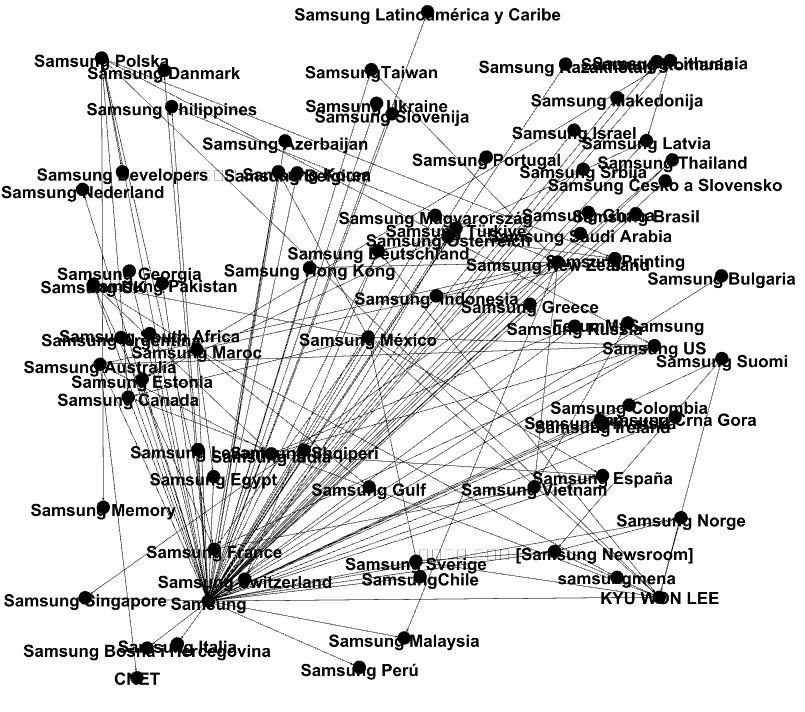
\includegraphics[width=0.7\textwidth]{photos-files/section3/first_painting.jpg}
		\end{center}
	\newpage
	
	Επίσης μέσω του Gephi μπορούμε να θέσουμε διάφορες παραμέτρους όσον αφορά τoν χρωμaτισμό και την διάταξη ανάλογα με ορισμένες ιδιότητες που έχει το δίκτυο μας. Για παράδειγμα, για τη μορφή των κόμβων θέσαμε το μέγεθος του κάθε κόμβου ανάλογα με το πλήθος των εγγραφών(subscribercount) που έχει το κανάλι που αντιπροσοπεύει και για τον χρωματισμό θέσαμε ασπρο-πορτοκαλι-κοκκινο στο χαρακτηριστικο των προβολών(viewcount(100s)). Για την διάταξη, τρέξαμε τον Atlas Force 2 για να αραιώσουμε τον γράφο μας και τον Label Adjust για να διαχωριστουν οι ετικέτες ονομάτων των κόμβων. Έτσι προέκυψε η πάρακάτω εικόνα:
		\begin{center}
			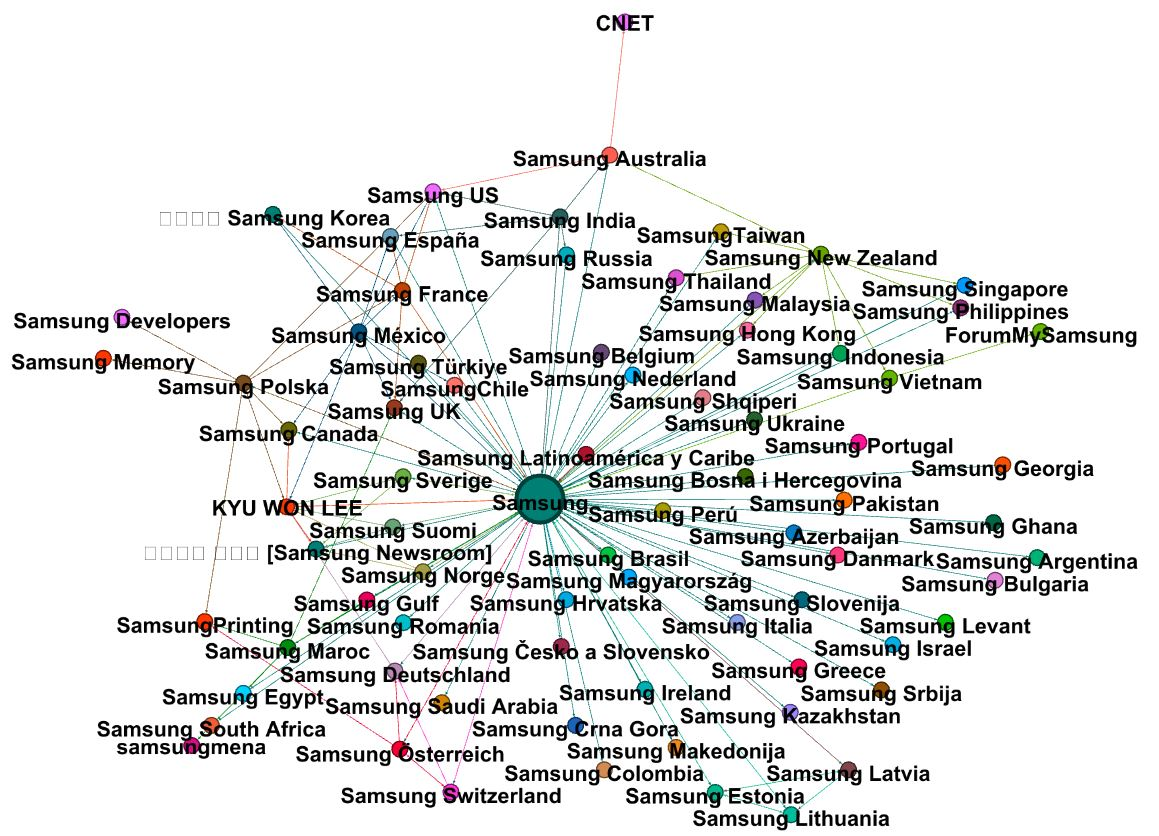
\includegraphics[width=0.8\textwidth]{photos-files/section3/second_painting.jpg}
		\end{center}
	Απο την εικόνα αυτή, τα δεδομένα που λαμβάνουμε είνα ο αριθμός των εγγραφών σε ενα κανάλι παίζει αρκετό ρόλο με τις προβολές που μπορεί να εχει, πραγμα αναμενόμενο για τον ιστότοπο που συζητάμε.
	\newpage
	
	Βλέποντας τα δεδομένα του δικτύου μας απο το Data Laboratory του Gephi, παρατηρήσαμε πως υπάρχουν κανάλια απο διάφορες χώρες. Επομένως θεωρήσαμε ενδιαφέρον να κάνουμε μία παραμετροποίηση με τις χώρες ως εξής. Ο χρωματισμός έγινε μέσω διφορετικών χρωματων, τοσων, όσος και ο αριθμός των διαφορετικών χωρών, μέσω του partition tab. Στο σημείο αυτο, θεώρήσαμε επίσης σημαντικό και την αναφορά του seed. Αυτό έγινε μεσω του μεγέθους των κόμβων μέσω του seedrank(αντίστοιχη μεταβλητη με την isseed εαν χρησιμοποιούσαμε τον χρωματισμό). Στη συνέχεια μέσω του Plugin Circular Layout που κατεβάσαμε μέσω των Tools του Gephi, δημιουργήσαμε την πιο κάτω διάταξη θέτοντας στην ιδιότητα "Order Nodes By" την χώρα. Για άλλη μια φορά, χρησιμοποιήσαμε τον Label Adjust για διαχωρισμό των ετοικετών.
		\begin{center}
			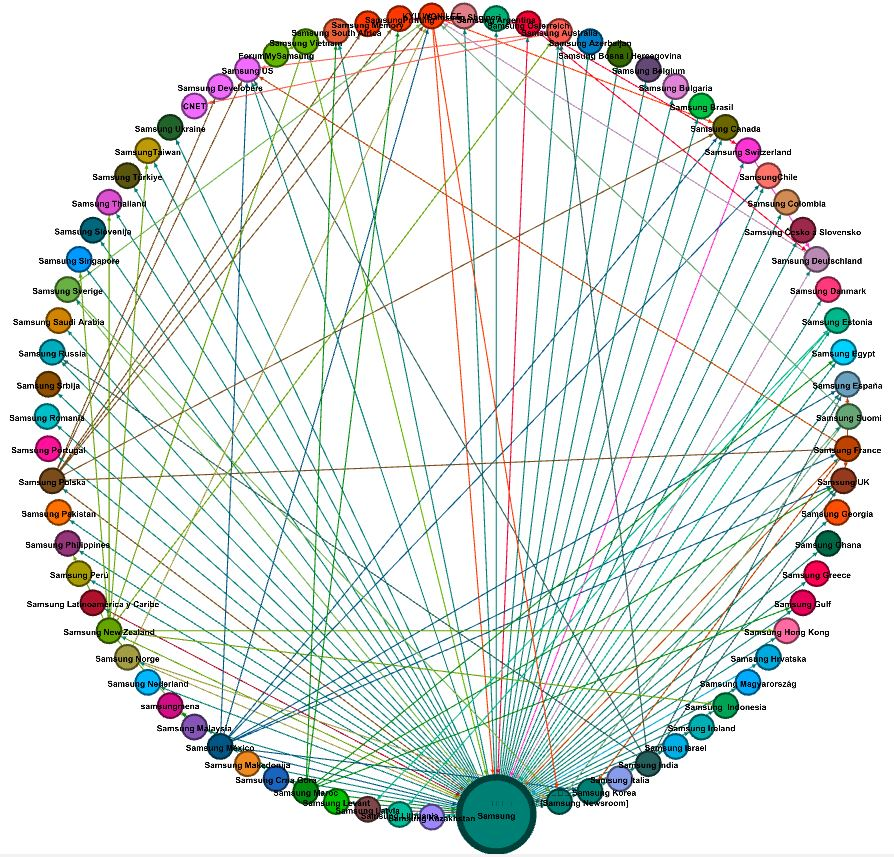
\includegraphics[width=0.8\textwidth]{photos-files/section3/third_painting.jpg}
		\end{center}
	Απο την πιο πάνω εικόνα μπορούμε εύκολα να παρατηρήσουμε πως ο κεντρικός και ισως ο πιο σηαντικος κόμβος να είναι ο "Samsung" ο οποίος είναι με πράσινο χρώμα. Οι δύο δεξιές θέσεις απο αυτο το κόμβο είναι επίσης με πράσινο χρώμα αφού και αυτοι οι κόμβοι είναι κανάλια απο την ίδια χώρα, την Νότιο Κορέα.
	\label{chap:graphical_representation_3}
	
	
	\section{Βασικά στοιχεία Δικτύου}
	Το δίκτυο που μελετάμε έχει τα εξής βασικά στοιχεία:
	\begin{itemize}
		\item Αριθμός κόμβων: \textbf{76} διαφορετικά \textbf{κανάλια-κόμβοι}
		\item Αριθμός ακμών: \textbf{149 συνδέσμοι} μέσω των οποίων συνδέονται τα κανάλια-κόμβοι
		\item Ο γράφος μας είναι \textbf{κατευθυνόμενος}. Δηλαδή κάθε σύνδεσμος απο ενα κανάλι προς ενα άλλο εχει κατέυθυνση όπως φαινεται στην πιο κάτω εικόνα:
		\begin{center}
			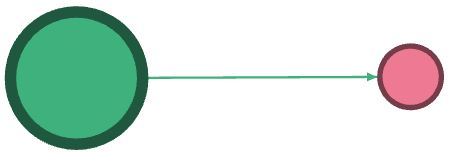
\includegraphics[width=0.8\textwidth]{photos-files/section4/ate.JPG}
			
			Ο πράσινος κόμβος-κανάλι έχει ως featured channel τον κόμβο-κανάλι με ροζ χρώμα.
		\end{center}
		\item Διάμετρος δικτύου: Η \textbf{διάμετρος} ενός δικτύου είναι η μακρύτερη συντομότερη διαδρομή που μπορούμε να βρούμε. Στην περίπτωσή μας είναι \textbf{3}. Τιμή αναμενόμενη λόγω του depth με τιμή 2 που επιλέξαμε.
		\item \textbf{Average path length}: Είναι ο \textbf{μέσος όρος των συντομότερων μονοπατιών} για όλα τα ζεύγη κόμβων. Στο δίκτυο μας είναι \textbf{1.9760}.
		\begin{center}
			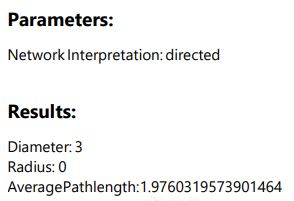
\includegraphics[width=0.4\textwidth]{photos-files/section4/graph_distance_report.JPG}
		\end{center}
	\end{itemize}
	\label{chap:basic_network_elements_4}
	
	
	\newpage
	\section{Component Measures}
	Στο δίκτυο μας, όλοι οι κόμβοι είναι συνδεδεμένοι μεταξύ τους(έμμεσα είτε άμεσα). Άρα μπορούμε να πούμε πως υπάρχει \textbf{ένα giant component}. Επομένως ο αριθμός των \textbf{weakly connected components} είναι ίσος με \textbf{1}. \par 
	Αναφορίκα με τον αριθμό των \textbf{strongly connected components}, αυτό που πρέπει να δούμε στην περίπτωση μας είναι αν υπάρχουν κανάλια-κόμβοι τα οποία δεν έχουν Featured Channels, δηλαδή δεν έχουν εξερχόμενους συνδέσμους. Έτσι μέσω του Connected Components tool απο το πεδίο Statistics του Gephi έχουμε την ακόλουθη αναφορά.
	\par
	\begin{center}
		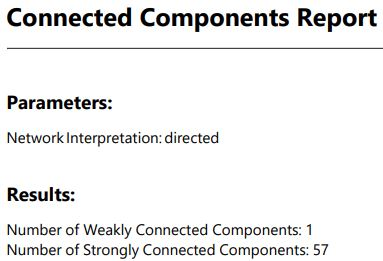
\includegraphics[width=0.4\textwidth]{photos-files/section5/connected_components_report.JPG}
	\end{center}
	\par
	Παρατηρόντας την πιο πάνω είκονα λοιπόν, μπορούμε να επιβεβαιώσουμε τον αριθμό των weakly connected components. Όσον αφορά τον αριθμό των strongly connected components μεσω του Gephi βλέπουμε πως είναι \textbf{57}. Στο σημείο αυτο μπορούμε να εφαρμόσουμε μια διάταξη για να δούμε σχηματικά αυτους τους κόμβους ώστε να καταλάβουμε καλύτερα τι σημβαίνει. Χρησιμοποιόντας λοιπόν τον αλγόριθμο Dual Circle Layout, με Upper Order Count ίσο με 20(Πλήθος κόμβων - strong connected components + weakly connected components) με σκοπό να πάρουμε στον εξωτερικό κύκλο τα κανάλια που δεν έχουν Featured Channels(20 κανάλια, 20 διαφορετικά χρώματα). Έτσι όπως φαίνεται και πιο κάτω, στον εξωτερικό κύκλο, τα κανάλια αυτά έχουν ακμές που φτάνουν σε αυτά και κανένα δεν έχει ακμή που να ξεκινάει απο αυτά.
	\begin{center}
		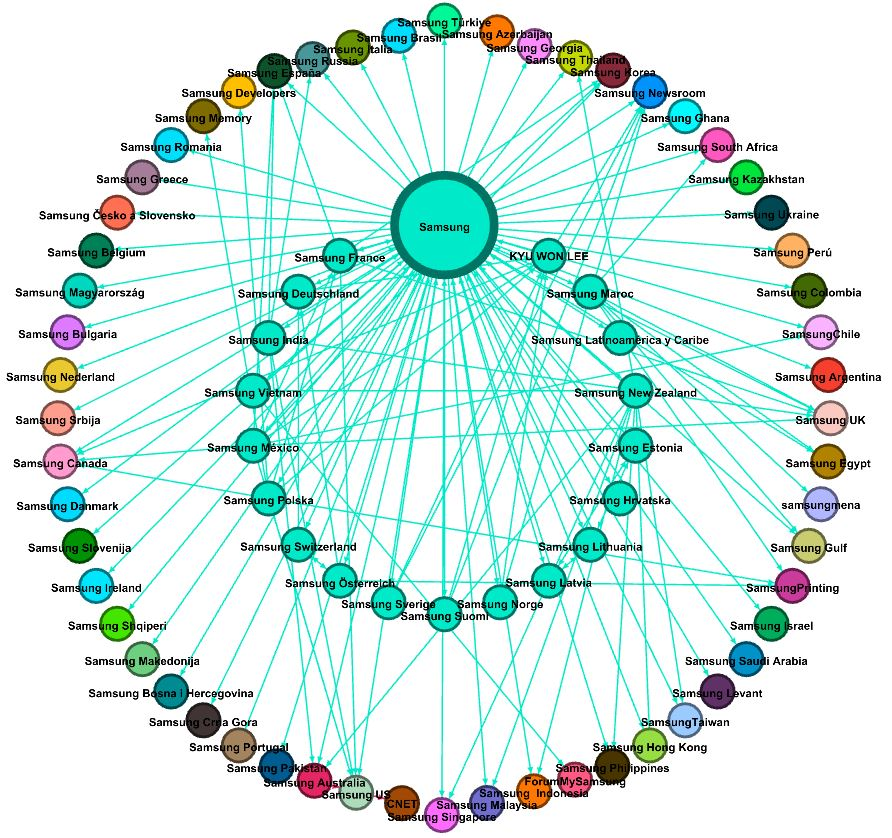
\includegraphics[width=0.8\textwidth]{photos-files/section5/section5_photo1.JPG}
	\end{center}
	Να σημειωθεί οτι κρατήσαμε διαμόρφωση των κόμβων σχετκα με το μέγεθος στην σχέση seedrank χωρις αυτο να παιζει κάποιο ρόλο, γι'αυτο και ο κόμβος Samsung έχει μεγαλύτερο μέγεθος.
	\label{chap:component_measures_5}
	
	
	\newpage
	\section{Degree Measures}
	\textcolor{red}{(mikri eiagogi AN DEN FKENNEI EN OK)Στο σημέιο αυτό της analisis mas tha aaferthoume sta degree measures. ta degree measures einai...}
		
	\subsection{Maximum Degree}
	Το Maximum Degree είναι ο μέγιστος αριθμός ακμών που έχει ενας κόμβος μέσα στο δίκτυο. Στην περίπτωση που εξετάζουμε, αφορά τον κόμβο "Samsung" με τιμη 87. Αποτέλεσμα αναμενόμενο, αφού ο συγκεκριμένος κόμβος παίζει τον πιο σηαντικό ρόλο στο δίκτυο μας όπως έχουμε δεί και σε αλλες παριπτώσεις. Αυτό φαίνεται μέσω του πιο κάτω στιγμιότυπου που πηραμε απο το Gephi αφού βρήκαμε πρώτα το degree του κάθε κόμβου.
	\begin{center}
		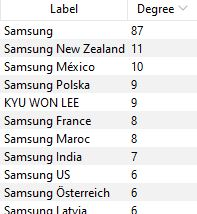
\includegraphics[width=0.3\textwidth]{photos-files/section6/maximum_degree.JPG}
	\end{center}
	
	\subsection{Average Node Degree}
	Το Average Node Degree είναι ο μέσος αριθμός ακμών που υπάρχουν στο δίκτυο. Στο δίκτυο μας είναι ίσο με 1.961 σύμφωνα με το Degree Report που φτιάξαμε μέσω του Gephi απο το μενού Statistics.
	\begin{center}
		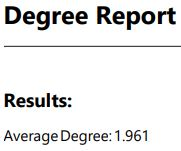
\includegraphics[width=0.2\textwidth]{photos-files/section6/average_degree.JPG}
	\end{center}
	
	\newpage
	\subsection{Degree Distribution} % --------------------------------------------------- Degree Distribution
	\textcolor{red}{isos na valw mia mikri isagogi?}
	
	\subsubsection{In-Degree} % ---------------------------------------------- In-Degree
	Το In-Degree είναι οι εισέρχόμενες προς κάποιον κόμβο ακμές. Στην περίπτωση μας, ο αριθμος αυτός αποτελεί τον αριθμό των καναλιών που έχουν ως Featured Channel το κανάλι που εξετάζουμε. Έτσι για κάθε κανάλι με τη βοήθεια του Gephi για το δίκτυο μας έχουμε:		
	\begin{center}
		\begin{adjustbox}{valign=t, valign=}
			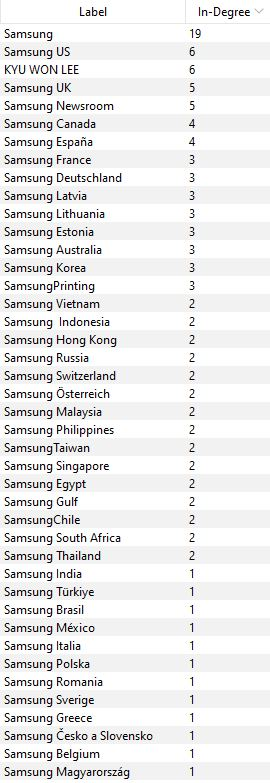
\includegraphics[width=0.34\textwidth]{photos-files/section6/in-degree1.JPG}
		\end{adjustbox}
		\hfill
		\begin{adjustbox}{valign=t}
			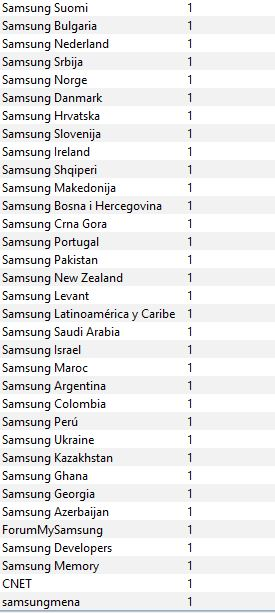
\includegraphics[width=0.34\textwidth]{photos-files/section6/in-degree2.JPG}
		\end{adjustbox}
	\end{center}
	\newpage
	Κατανομή του In-Degree μέσω γραφικής παράστασης:
	\begin{center}
		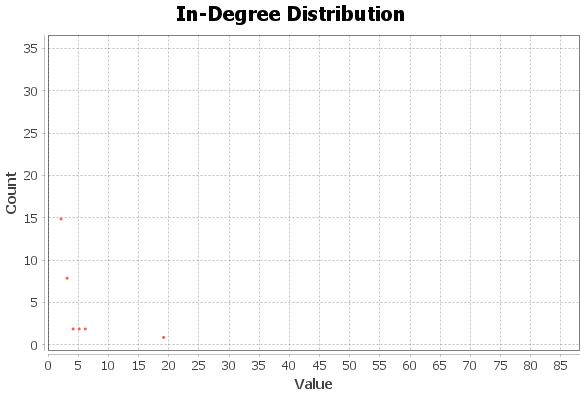
\includegraphics[width=0.7\textwidth]{photos-files/section6/in-degree_graphical.JPG}
	\end{center}
	Μετά απο τα πιο πάνω, θα ήταν αρκετα ενδιαφέρον να δούμε πως αλλάζει το δίκτυο όσον αφορά μέγεθος και χρώμα κόμβων σε σε συνάρτηση με το In-Degree.\textcolor{red}{dipla pou thn pio katw na mpei h ipolipi ths}
	\begin{center}
		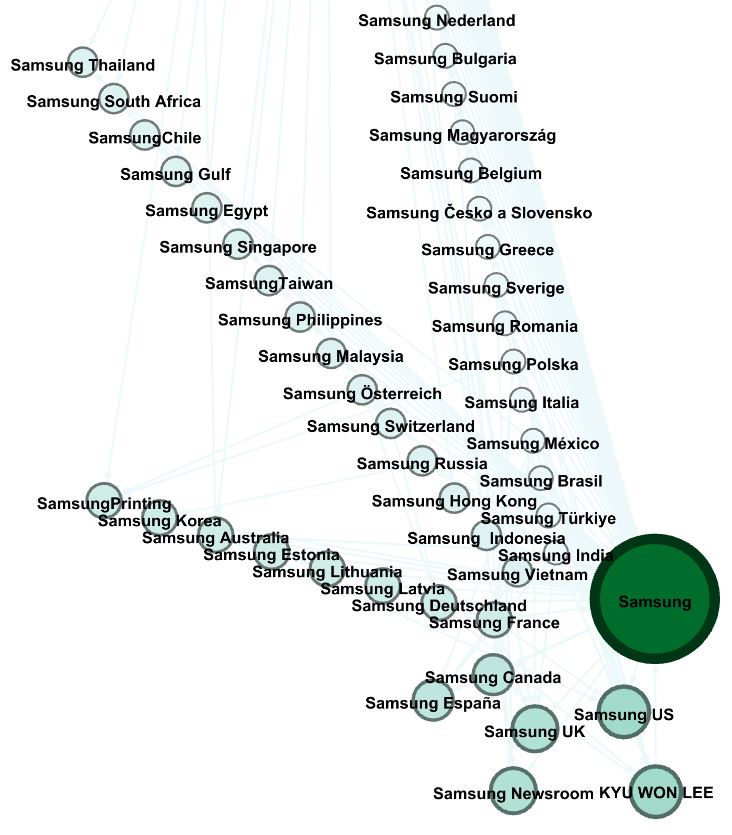
\includegraphics[width=0.6\textwidth]{photos-files/section6/in-degree_RE-layout.JPG}
	\end{center}
	Έτσι χρησιμοποιόντας τον αλγόριθμο Radial Axis Layout μπορούμε να δούμε τον διαχωρισμο που γινεται ανάμεσα στους κόμβους σε σχέση με το in-degree του κάθε καναλιού. Τα κανάλια λοιπόν χωρήστκαν σε 7 διαφορετικές ομάδες σε οριζόντιους άξονες αφου οι διαφορετικές τιμες που παρατηρούνται είναι 7 όπως είδαμε και στους πιο πάνω πίνακες. Έτσι στο σημείο αυτό μπορούμε εύκολα να δούμε τα κανάλια τα όποια υπάρχουν κατα πολυ περισσότερες φορές ως Featured channels σε άλλα. Προταγωνησικο ρόλο έχει το κανάλι της Samsung για ακόμα μια φορα ενω ακολουθούν στη συνέχια τα κανάλια SamsungUS,  KYO WON LEE κοκ.
	
	\subsubsection{Out-Degree} % -------------------------------------------- Out-Degree
	Το Out-Degree είναι οι εξέρχόμενες απο τον κάθε κόμβο ακμές. Με το δίκτυο το οποίο μελετάμε είναι ο αριθμός των Featured Channels που μπορεί να έχει ένα κανάλι όπως βλέπουμε παρακάτω.
	\begin{center}
		\begin{adjustbox}{valign=t}
			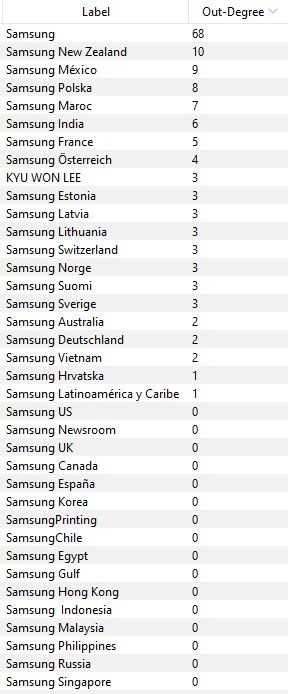
\includegraphics[width=0.34\textwidth]{photos-files/section6/out-degree1.JPG}
		\end{adjustbox}
		\hfill
		\begin{adjustbox}{valign=t}
			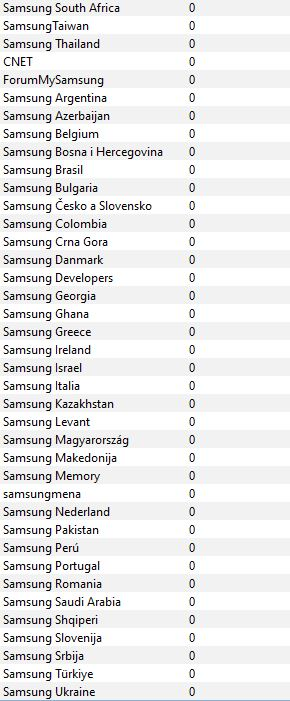
\includegraphics[width=0.34\textwidth]{photos-files/section6/out-degree2.JPG}
		\end{adjustbox}
	\end{center}
	\newpage
	Κατανομή του Out-Degree μέσω γραφικής παράστασης:
	\begin{center}
		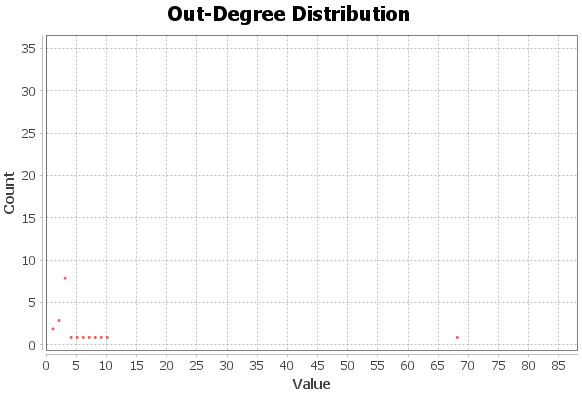
\includegraphics[width=0.7\textwidth]{photos-files/section6/out-degree_graphical.JPG}
	\end{center}
	Αντίστοιχα με το In-Degree θα δούμε πως αλλάζει το δίκτυο όσον αφορά μέγεθος και χρώμα κόμβων σε συνάρτηση με το Out-Degree αυτη τη φορά.\textcolor{red}{dipla pou thn pio katw na mpei h ipolipi ths}
	\begin{center}
		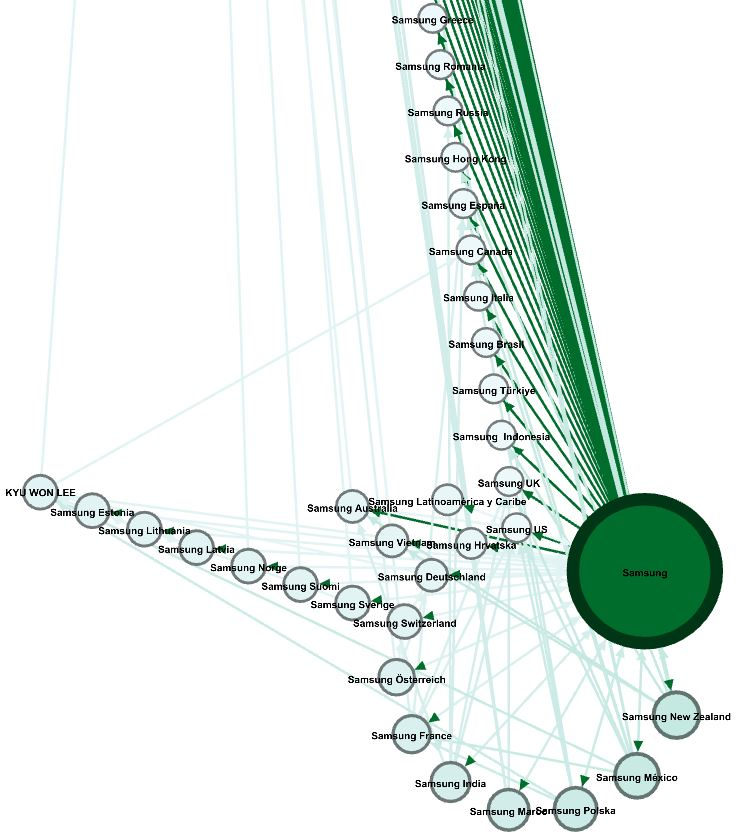
\includegraphics[width=0.6\textwidth]{photos-files/section6/out-degree_RE-layout.JPG}
	\end{center}
	Με τον αντίστοιχο τρόπο που δουλέψαμε για το In-Degree προηγουμένως, δουλέψαμε και τώρα. Όπως παρατη- ρούμε, στην πρωτη θέση εξακολουθει να είναι το καναλι Samsung ενω στο προσκήνιο έχουν προστεθει αρκετα κανάλια σε σχέση με πριν. Λογικό, αφου όσο πιο πολλα Featured Channels έχει ενα κανάλι τοσο πιο εύκολα μπορεί να προσεγγίσει κοινό και να αυξήσει τις προβολές και τις εγγραφές του. Επίσης ένα παράδειγμα που πολλές φορες συμβαίνει είναι οτι με αυτον τον τρόπο ο κόσμος μπορεί να ενημερωθεί πολυ πιο γρήγορα για ενα καινούργιο προιον που έχει παρουσιαστει σε μια άλλη χωρα βλέποντας ενα προτεινόμενο κανάλι που θα προτείνει η ίδια η πλατφόρμα του YouTube μέσω των Featured Channels που έχει το κανάλι το οποίο ακολουθεί ένας χρήστης.
	
	\newpage
	\subsubsection{Total Degree} % ------------------------------------------ Out-Degree
	Το Total Degree είναι το σύνολο των ακμών που ξεκηνούν ή που καταλήγουν σε ένα κόμβο. Με άλλα λόγια, είναι ουσιαστικά το άθροισμα του In-Degree και του Out-Degree.
	\begin{center}
		\begin{adjustbox}{valign=t}
			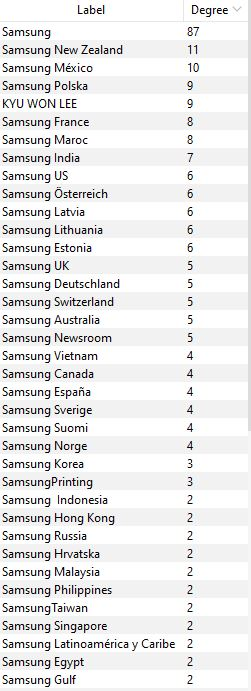
\includegraphics[width=0.34\textwidth]{photos-files/section6/total-degree1.JPG}
		\end{adjustbox}
		\hfill
		\begin{adjustbox}{valign=t}
			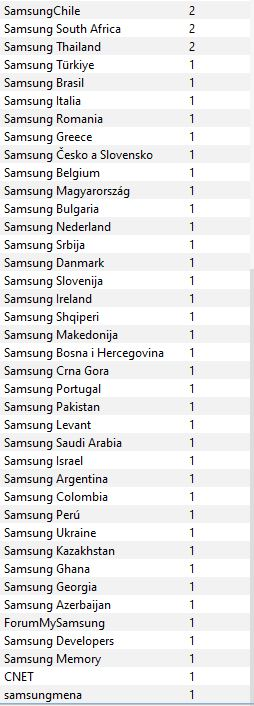
\includegraphics[width=0.34\textwidth]{photos-files/section6/total-degree2.JPG}
		\end{adjustbox}
	\end{center}
	\newpage
	Κατανομή του Total Degree μέσω γραφικής παράστασης:
	\begin{center}
		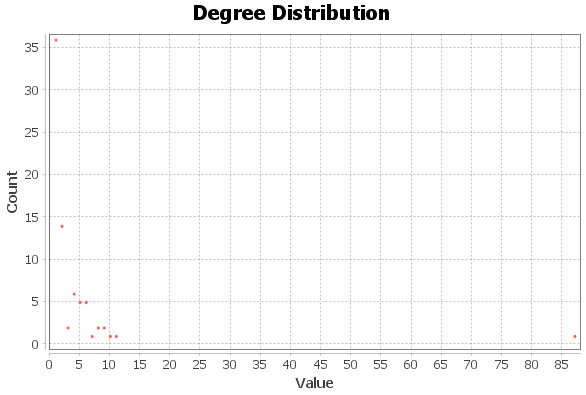
\includegraphics[width=0.7\textwidth]{photos-files/section6/total-degree_graphical.JPG}
	\end{center}
	Όπως και στις δύο προηγούμενες περιπτώσεις, θα δούμε πως διαμορφώνεται το δίκτυο μας λαμβάνοντας υπόψην το Total Degree αυτή τη φορά. \textcolor{red}{dipla pou thn pio katw na mpei h ipolipi ths}
	\begin{center}
		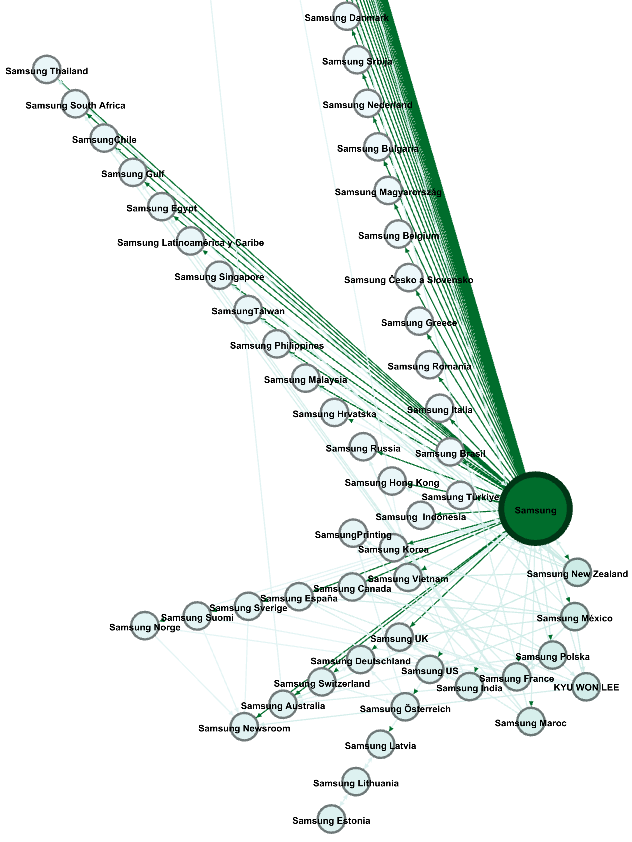
\includegraphics[width=0.5\textwidth]{photos-files/section6/total-degree_RE-layout.png}
	\end{center}
	\par
	Το πρώτο πράγμα που μπορεί να προσέξει κανεις για το σχήμα που προέκυψε με μετρική το Total Degree είναι πως υπάρχει ο ίδιος αριθμός ομάδων κατα πλήθος κόμβων σε σχέση με πριν. Η διαφορά όμως έγγυται στο γεγονός πως όλοι σχεδόν οι κόμβοι που υπήρχαν και πριν στο Out-Degree, πέραν απο τον προφανές της Samsung, υπάρχουν και τώρα. Άρα φαίνεται πως το Out-Degree είναι αυτο που παίζει τον πιο σημαντικό ρόλο αφού όπως είπαμε και προηγουμένως είναι αυτό που καθορίζει ποια κανάλια θα προωθηθούν περισσότερο απο τον τρόπο που δουλεύει το Youtube μέσω των Featured Channels.
	\vspace{12pt}
	\par
	Τέλος να πούμε πως δεν έγινε κάποια αναφορά για το Weight Degree αφου στο δίκτυο που μελετάμε όλες οι ακμές έχουν ίσο βάρος πραγμα που δεν επηρεάζει τα δεδομένα μας. Επομένως δεν είχε νόημα η οποιαδίποτε αναφορά σε αυτό. \textcolor{red}{sioureftou full gia touto an j nmz en k dioti j sto fire etsi elalen}
	\label{chap:degree_measures_6}
	
	
	
	
	
	\newpage
	\section{Centrality measures}
	
	\subsection{Degree}
	\textcolor{red}{dame enikserw ti na grapsw, sthn ekfonisi lalei gia Degree enw sto Section6 pou en ta Degree Measures lalei gia Total Degree. enen idia touta ta 2? na mpw stes dialeksis gia to section7 na dw ti lalei}
	
	\subsection{Betweenness Centrality}
	Το Betweenness Centrality δείχνει πόσο σημαντικός είναι ένας κόμβος(ως ενδιάμεσος) όταν θέλουμε να συνδέσουμε όλους τους κόμβους μεταξύ τους μέσω αυτού. Για παράδειγμα, για τον κόμβο \(n_i\) βρίσκουμε για κάθε ζεύγος κόμβων(u, w) του δικτύου τις εξής τιμές όπου και τις διαιρούμε:
	\begin{enumerate}
		\item Το σύνολο των συντομότερων μονοπατιών απο τον κόμβο \(n_i\): \( \Sigma_{u \omega}(n_i) \)
		\item Με τον αριθμο των συντομότερων διαδρομων που παιρνούν απο τον κόμβο x(τα μονοπάτια των u προς w):\( \Sigma_{u \omega} \)
	\end{enumerate}
	Αθροίζοντας το πηλίκο των διαιρέσεων των σημείων 1 και 2 βρίσκουμε το Betweenness Centrality του κόμβου x.
	Ο τύπος για την πιο πάνω διαδικάσια δίνεται απο την σχέση \(C_B(n_i)\) = $\sum$(\( \Sigma_{u \omega}(n_i) \) / \( \Sigma_{u \omega} \)).
	% https://www.youtube.com/watch?v=PuWNYB0u_gM
	
	\vspace{12pt}
	\vspace{12pt}
	Αφού καταλάβαμε πως προκύπτει το Betweenness Centrality, μπορούμε με την χρήση του Gephi να το βρούμε αυτόματα για όλους τους κόμβους μέσω των Statistics.
	\begin{center}
		\begin{adjustbox}{valign=t}
			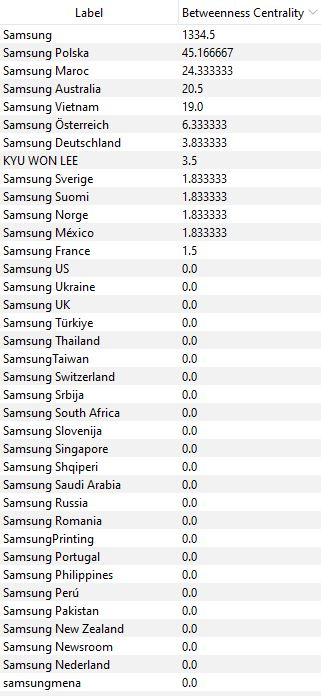
\includegraphics[width=0.4\textwidth]{photos-files/section7/betweenness_centrality1.JPG}
		\end{adjustbox}
		\hfill
		\begin{adjustbox}{valign=t}
			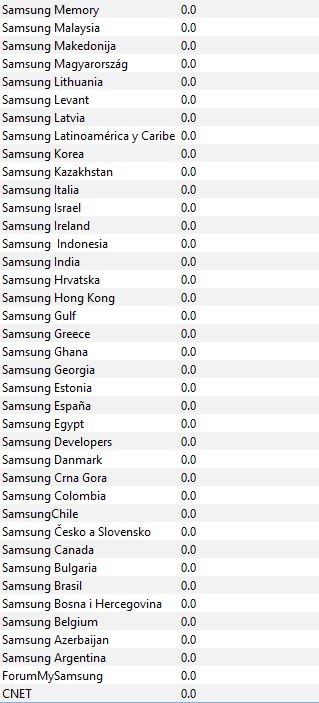
\includegraphics[width=0.4\textwidth]{photos-files/section7/betweenness_centrality2.JPG}
		\end{adjustbox}
	\end{center}
	\vspace{12pt}
	Όπως φαίνεται και απο τους πιο πάνω πίνακες λοιπόν, είναι λίγες οι χώρες που έχουν μη μηδενικό Betweenness Centrality. Στην κορυφή των μετρήσεων μας είναι για ακόμη μια φορα το κανάλι της Samsung ενώ έχουν ανέβει στην κορυφή τώρα ορισμένα κανάλια όπου σε προηγούμενες μετρλησεις δεν ήταν σε τόσο υψηλή θέση. %Παραδείγματα τέτοιων καναλιών είναι τα Samsung Polska(Πολωνία), Samsung Maroc, Samsung Australia, Samsung Vietnam, Samsung Osterreich(Αυστρία), \textcolor{red}{eksiasa thn india} Samsung Deutschland(Γερμανία), Samsung Sverige(Σουηδία), Samsung Suomi(Φινλανδία), Samsung Norge(Νορβηγία), Samsung Mexico και Samsung France. 
	Όπως βλέπουμε, υπάρχουν μία ή περισσότερες χώρες απο κάθε ήπειρο εκτός απο την Ευρώπη που συγκεντρώνει 7 χώρες.
	
	\newpage
	\subsection{Closeness Centrality}
	Το Closeness Centrality είναι μια μετρηκη που αποσκοπέι στο πόσο κοντά είναι ένας κόμβος σε όλους τους άλλους. Να σημειωθεί επίσης οτι μικρότεροι αριθμοί δείχνουν πως ένας κόμβος έχει υψηλό Closeness Centrality με τις τιμές να κειμένονται απο 0 εως 1.
	\par
	Τον τρόπο με τον οποίο μπορούμε να υπολογίσουμε τη μετρικλη αυτή σε ένα κατευθυνόμενο δίκτυο όπως το δικό μας μπορούμε να τον δούμε μέσω του ακόλουθου παραδείγματος.
	\begin{center}
		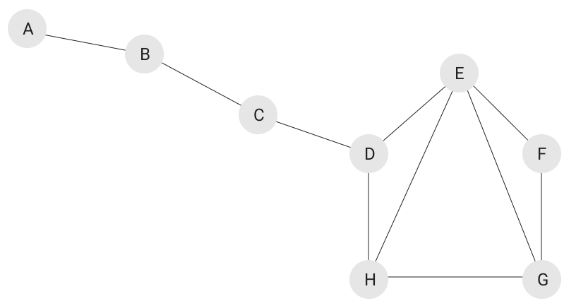
\includegraphics[width=0.5\textwidth]{photos-files/section7/closeness_centrality_example.JPG}
	\end{center}
	Έστω πως θέλουμε να βρούμε το Closeness Centrality για τον κόμβο C. Βρίσκουμε τον συνολικό αριθμό αριθμό κόμβων του δικτύο μας και αφαιρούμε ένα, και τον διαιρούμε με το άθροισμα των συντομότερων μονοπατιών απο τον κόμβο που εξετάζουμε προς όλους τους υπόλοιπους. Επομένως για τον κόμβο C έχουμε:
	\begin{center}
		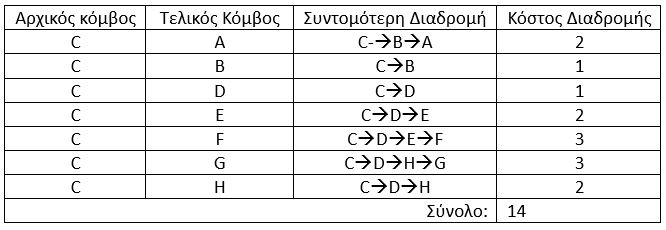
\includegraphics[width=0.7\textwidth]{photos-files/section7/array_of_example.JPG}
	\end{center}
	Άρα το Closeness Centrality του κόμβου C είναι 7/14 = 0.5
	\par
	Να πούμε επίσης πως σε κατευθυνόενους γράφους, παίζει ρόλο η φορά των ακμών. Για παράδειγμα σε περιπτωσεις όπου δεν υπάρχει διαδρομή λόγω φοράς ακμών, θεωρούμε μηδενικό το μονοπάτι. Έτσι γενικέυοντας το πιο πάνω υπάρχει περίπτωση κάποιος κόμβος να έχει μηδενικό Betweenness Centrality.
	
	\newpage
	Τώρα με την βοήθεια του Gephi μέσω των Statistics έχουμε τις εξής τιμές για τη μετρική αυτή.
	\vspace{12pt}
	\begin{center}
		\begin{adjustbox}{valign=t}
			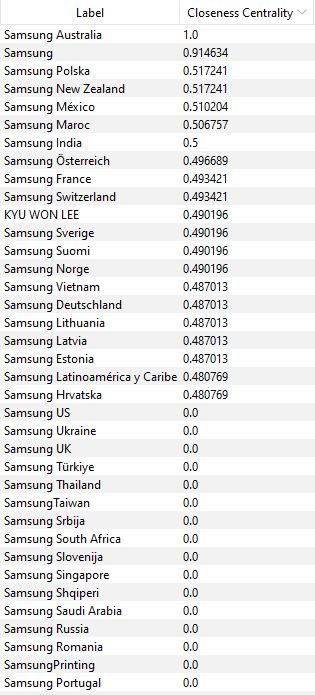
\includegraphics[width=0.4\textwidth]{photos-files/section7/closeness_centrality1.JPG}
		\end{adjustbox}
		\hfill
		\begin{adjustbox}{valign=t}
			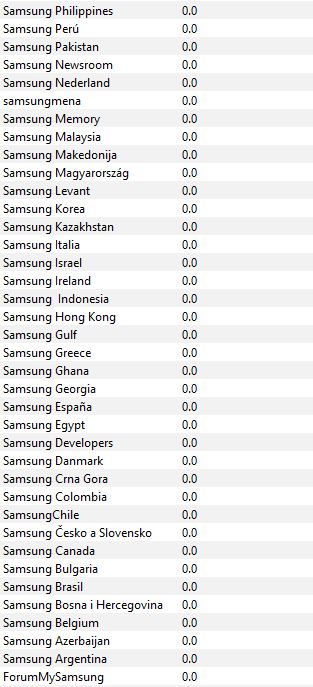
\includegraphics[width=0.4\textwidth]{photos-files/section7/closeness_centrality2.JPG}
		\end{adjustbox}
	\end{center}
	
	\newpage
	Παρατηρόντας τις πιο πάνω τιμές βλέπουμε πως υπάρχει μια κατανομή για το Closeness Centrality των καναλιών του δικτύου μας. Έτσι για να καταλάβουμε καλύτερα τι συμβαίνει μπορούμε να δούμε τις τιμές αυτές μέσω του ακόλουθου διαγράμματος.
	\vspace{12pt}
	
	\begin{center}
		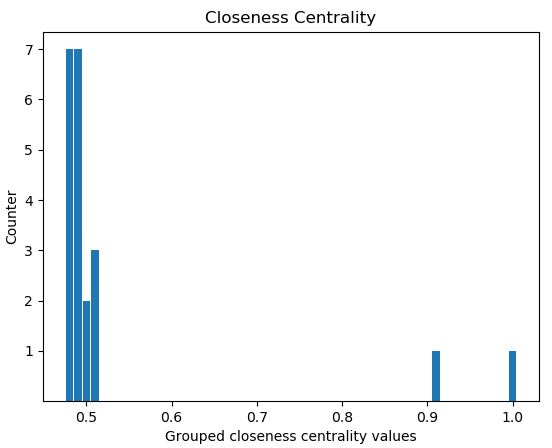
\includegraphics[width=0.7\textwidth]{photos-files/section7/bar_chart_for_7.3.JPG}
	\end{center}
	Βλέπουμε λοιπόν πως υπάρχει μια ομαδοποίηση των κόμβων μεταξύ των τιμών 0.48 και 0.51. Αντίθετα όμως, μόνο δύο κόμβοι έχουν υψηλές τιμές της τάξης των 0.91 και 1.0. Άρα αμέσως καταλαβαίνουμε οτι τα κανάλια που έχουν πιο σημαντικό ρόλο στο δίκτυο μας είναι αυτα με 0.91 και 1.0 με το όνομα αυτων να ειναι Samsung και Samsung Australia αντιστοιχα. Στο σημείο αυτό, να σημειωθεί οτι υπάρχουν αρκετά κανάλια τα οποία έχουν μηδενικό Closeness Centrality αφού είναι κανάλια τα οποία είναι featured channels άλλων καναλιών ενω ταυτόχρονα τα κανάλια αυτά δεν εχουν δικά τους featured channels.
	
	
	\newpage
	\subsection{Eigenvector Centrality}
	Το Eigenvector Centrality είναι ένα μετρο με το οποίο μπορούμε να καταλάβουμε την επηροή που μποροεί να έχει ένας κόμβος μέσα στο δίκτυο μας. Δείχνει δηλαδή πόσο σημαντικός είναι ένας κόμβος ανάλογα με το ποσο σημαντικοι είναι και οι κόμβοι-γειτονες που έχει.
	\par
	Ο τρόπος με τον οποίο μπορούμε να υπολογίσουμε τη μετρική αυτή σε ένα κατευθυνόμενο δίκτυο όπως το δικό μας μπορούμε να τον δούμε μέσω του εξής παραδείγματος. Έστω το ακόλουθο δίκτυο:
	% https://www.youtube.com/watch?v=IIBOT3SjJZE
	\begin{center}
		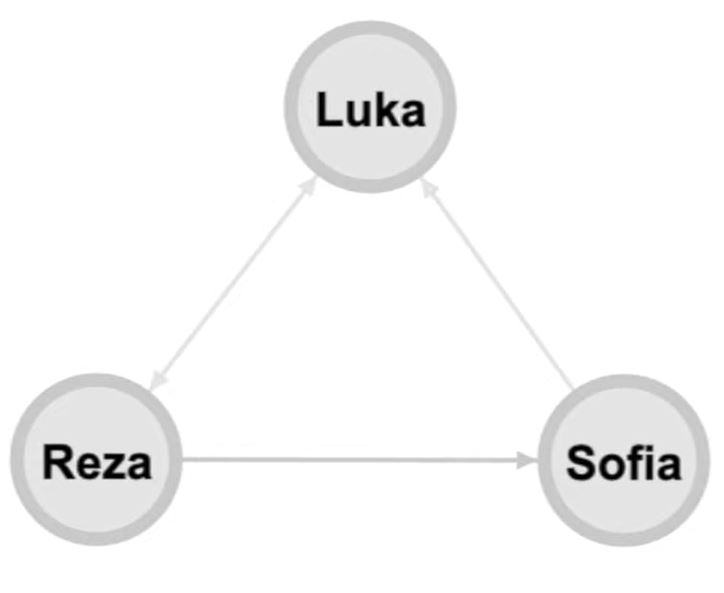
\includegraphics[width=0.4\textwidth]{photos-files/section7/eigenvector_entrality_example.JPG}
	\end{center}
	Αρχικά κατασκεύαζουμε το γραμμικό σύστημα(πίνακας δύο διαστάσεων) για το δίκτυο μας όπου βάζουμε τους αριθμούς 0 ή 1 εφόσον υπάρχει μονοπάτι που συνδέει τους κόμβους του δικτύου μας. Για παράδειγμα για τον κόμβο Reza η πρώτη στήλη στο γραμμικό μας σύστημα θα ειναι 0(θεωρούμε πως δεν υπάρχει μονοπατι απο κάποιο κόμβο προς τον εαυτό του), 1(για το μονοπάτι Reza προς Sofia) και 1(για το μονοπάτι Reza προς Luke). Έτσι, με αυτό το τρόπο προκύπτει ο ακόλουθος πίνακας.
	\begin{center}
		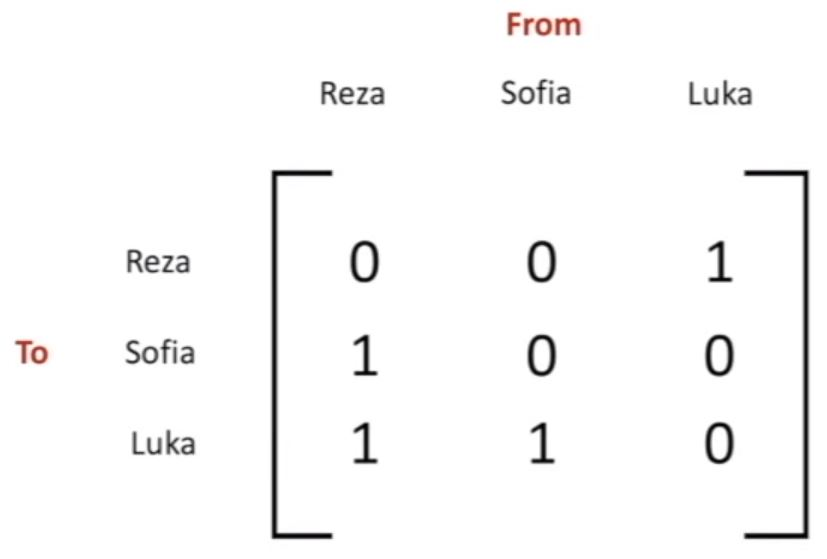
\includegraphics[width=0.5\textwidth]{photos-files/section7/eigenvector_entrality_examplev2.JPG}
	\end{center}
	
	\newpage
	Στη συνέχεια χρησιμοποιόντας αλγόριθμους γραμμικής άλγεβρας βρίκουμε το ιδιοδιάνυσμα που αντιστοιχεί στη μεγαλύτερη ιδιοτιμή του πίνακα που βρήκαμε στο προηγούμενο βήμα, κάνουμε κανονικοποίηση και έτσι προκύπτουν οι τιμες για το Eigenvector Centrality του κάθε κόμβου.
	
	\vspace{12pt}
	Τώρα με την βοήθεια του Gephi για το Eigenvector Centrality έχουμε τις εξής τιμές.
	\begin{center}
		\begin{adjustbox}{valign=t}
			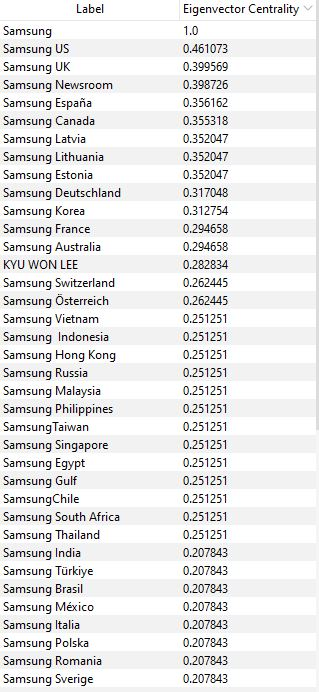
\includegraphics[width=0.4\textwidth]{photos-files/section7/eigenvector_centrality1.JPG}
		\end{adjustbox}
		\hfill
		\begin{adjustbox}{valign=t}
			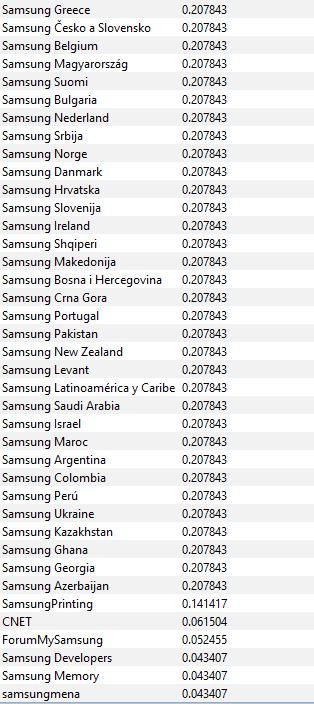
\includegraphics[width=0.4\textwidth]{photos-files/section7/eigenvector_centrality2.JPG}
		\end{adjustbox}
	\end{center}
	
	\newpage
	Αρχικά, το πρωτο πραγμα που βλέπουμε είναι πως δεν υπάρχουν μηδενικές τιμές σε αντίθεση με το Closeness Centrality αφου λαμβανοντας υπόψην τον αλγόριθμο με τον οποίο υπολογίζεται το Eigenvector Centrality όλοι οι κόμβοι είναι ενωμένοι με όλους έστω και με μία μονο ακμή.
	\par
	Πέραν απο το πιο πάνω, το πλέον σημαντικο που μπορουμε να πούμε για τα αποτελέσματα αυτά είναι πως υπάρχει μια μεγάλη αριθμιτική διαφορά μεαξυ του πρώτου σε σκόρ καναλιού και όλων των υπολοίπων. Στη πρώτη θέση λοιπόν βρίσκεται ξανα το κανάλι Samsung με σκόρ 1 ενώ τα υπόλοιπα κανάλια ξεκινουν απο σκόρ 0.46 και κάτω. Αυτο μας δείχνει οτι οι γείτονες των κόμβων μας είναι το ίδιο περίπου ισχυροι με μικρη διαφορα κάθε φορα που ολοενα και μικραίνει. Άρα φαίνεται πως επηρεάζονται περίπου το ίδιο κανάλια που βρισκονται ως featured channels σε άλλα αφού ο σκοπός είναι να φαίνονται όλα τα κανάλια χωρις να υπάρχει κάποιος ιδιαίτερος λόγος διαχωρισμού προτιμήσεων αφου στο δίκτυο που μελετάμε όλες οι συνδέσεις είναι με βαση το κρητηριο των featured channels.
	% https://www.youtube.com/watch?v=2bLD7yvy6jQ
	\label{chap:centrality_measures_7}
	
	
	\newpage
	\section{Clustering Effects}
	\subsection{Average Clustering Coefficient}
	Το Average Clustering Coefficient μας λέει την πιθανότητα με την οποία 2 γειτονικοι κόμβοι τυχαία επιλεγμένοι ενός τυχαίου κόμβου να είναι συνδεδεμένου. Ο τρόπος με τον οποίο υπολογίζουμε τη μετρική αυτή γίνεται ως εξής. Επιλέγουμε έναν τυχαό κόμβο όπου στη συnέχεια επιλέγουμε 2 γείτονες του τυχαία και στη συνέχεια ελέγχουμε εαν είναι συνδεδεμένοι. Αθροίζουμε τα αποτελέσματα της πάραπανω διαδικασίας για όλους τους κόμβους, διαιρούμε με το πλήθος των κόμβων και έτσι βρίσκουμε το επιθυμητό αποτέλεσμα. Στην περίπτωση μας με τη χρήση του Gephi βρίσκουμε πως το Average Clustering Coefficient για το δίκτυο μας είναι 0.311.
	\begin{center}
		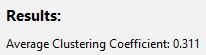
\includegraphics[width=0.4\textwidth]{photos-files/section8/average_clustering_coefficient.JPG}
	\end{center}
	
	\newpage
	\subsection{Number of Triangles}
	Ο όρος "Triangle" αναφαίρεται σε ένα σύνολο απο 3 κόμβους όπου κάθε κόμβος συνδέεαι με τους άλλους δύο. Για να υπολογίσουμε των συνολικό αριθμό τέτοιων συνόλων αρχικά θα πρέπει να θεωρήσουμε πως το δίκτυο μας είναι μη κατευθυνόμενο. Επομένως, μεσω του Gephi θα πρέπει να επιλέξουμε την αντίστοιχη επιλογή για μη κατευθυνόμενο γράφο. Τα αποτελέσματα λοιπόν φαίνονται πιο κάτω.
	\begin{center}
		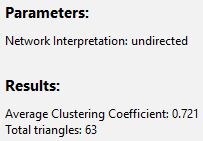
\includegraphics[width=0.4\textwidth]{photos-files/section8/number_of_triangles.JPG}
	\end{center}
	Απο το στιγμιότυπο που πήραμε απο το Gephi βλέπουμε αρχικά την ύπαρξη \textbf{63 Triangles}. Επίσης, παρατηρούμε πως έχει αλλάξει το Average Clustering Coefficient σε σχέση με πριν. Αυτό οφείλεται στο γεγονός ότι ο γράφος μας είναι μη κατευθυνόμενος με αποτέλεσμα να προσμετρούνται όλες οι συνδέσεις ανεξαρτήτος κατεύθυνσης. Επομένως 2 τυχαίοι γείτονες ενός τυχαίου κόμβου θα συνδέονται μεταξύ τους με πιθανότητα 0.721 έναντι 0.311 που ήταν προηγουμένως.
	\newpage
	Πιο κάτω φαίνονται αναλυτικότερα οι τιμες των Triangles ανα κανάλι.
	\begin{center}
		\begin{adjustbox}{valign=t}
			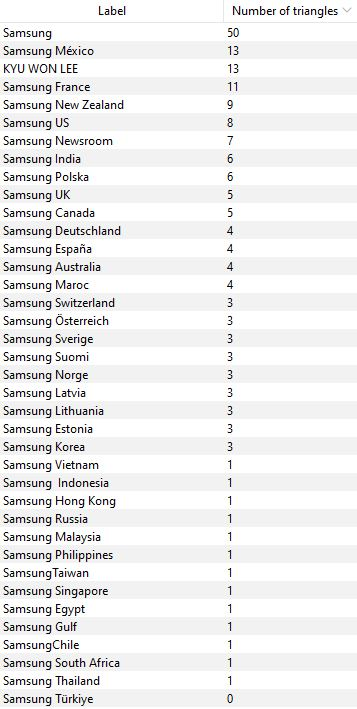
\includegraphics[width=0.4\textwidth]{photos-files/section8/num_of_triangles_1.JPG}
		\end{adjustbox}
		\hfill
		\begin{adjustbox}{valign=t}
			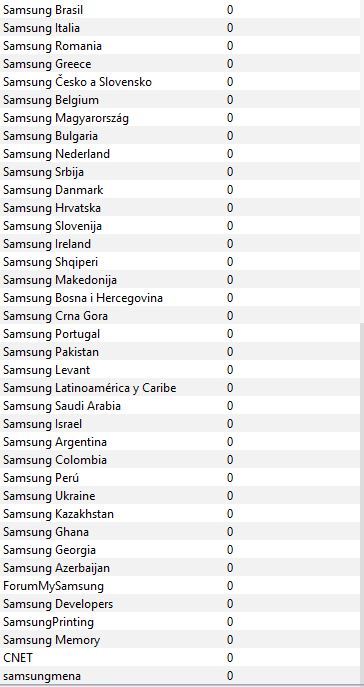
\includegraphics[width=0.4\textwidth]{photos-files/section8/num_of_triangles_2.JPG}
		\end{adjustbox}
	\end{center}
	\par
	Στο σημείο αυτό σκεπτόμενοι το γεγονός οτι παρόλο που εχουμε ενα κατευθυνόμενο δίκτυο έχουμε παράγει τα δεδομενα αυτα χωρις να λάβουμε υπόψην την κατέυθηνση των ακμών. Κατι τέτοιο κάναμε μονο στην ενότητα 7 όταν υπολογίσαμε το Total Degree αφου αθροίσαμε το In-Degree με το Out-Degree. Έτσι μέσω αυτής της παρατήρησης an anatreksoume stis antistoixes eikones pinakwn tha doume pws iparxei peripou h idia seira twn kanaliwn. \textcolor{red}{enikserw ti na grapsw dame...an grapsw thn idia paratirisi me ton allo en telia antigrafh meta opote na skeftw kati kalo}
	
	
	\newpage
	\subsection{Clustering Coefficient Distribution}
	Στο σημείο αυτό, μπορούμε να δούμε ξεχωριστά τις τιμές κάθε κόμβου για τη μετρική του Clustering Coefficient ξεκινόντας απο τη γραφική του Gephi.
	\begin{center}
		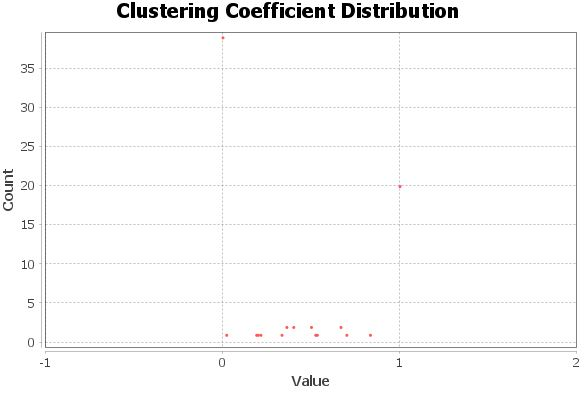
\includegraphics[width=0.7\textwidth]{photos-files/section8/distribution.JPG}
	\end{center}
	\par
	Όπως βλέπουμε οι τιμές είναι διάσκορπες στο διάστημα 0 εως 1 συμπεριλαμβανομένων, πράγμα που φαίνεται στην επόμενη σελίδα μέσω των δύο πινάκων.
	\begin{center}
		\begin{adjustbox}{valign=t}
			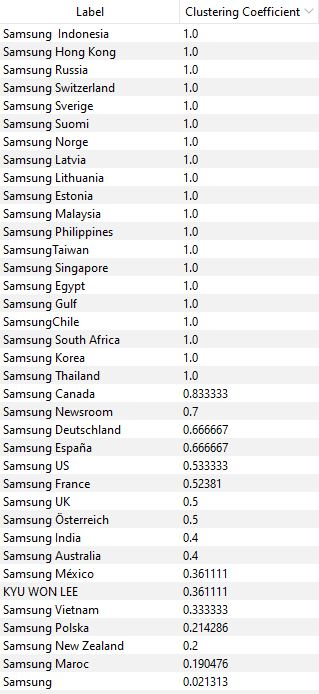
\includegraphics[width=0.4\textwidth]{photos-files/section8/distr_values1.JPG}
		\end{adjustbox}
		\hfill
		\begin{adjustbox}{valign=t}
			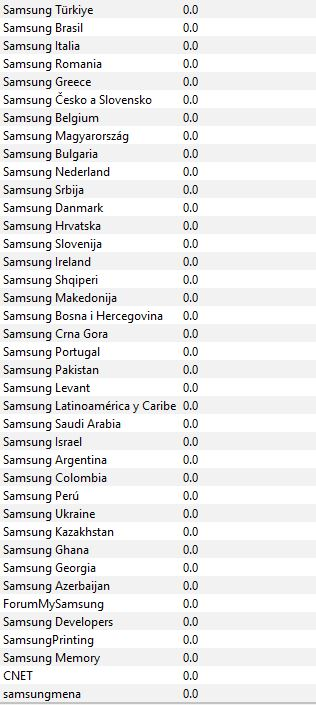
\includegraphics[width=0.4\textwidth]{photos-files/section8/distr_values2.JPG}
		\end{adjustbox}
	\end{center}
	Αντίθετα με τις υπόλοιπες μετρικές, τα αποτελέσματα δεν είναι συνηθισμένα. Κανάλια όπου σε προηγούμενες μετρικές είχαν υψηλό σκόρ τα βλέπυμε τώρα να έχουν χαμηλό, ενω κανάλια με χαμηλό σκόρ τώρα τα βλέπουμε να έχουν ψηλό Clustering Coefficient. Αυτό παρατηρείται ιδιαίτερα στα κοινωνικά δίκτυα αφου οι κόμβοι τείνουν να δημιουργούν στενά δεμένες ομάδες που χαρακτηρίζονται από σχετικά υψηλό Clustering Coefficient. Για παράδειγμα μπορούμε να δούμε κάποιες περιπτωσεις καναλιών για να καταλάβουμε πως σχηματίζονται οι ομάδες που αναφέραμε σε σχέση με το σκόρ του Clustering Coefficient.
	
	\newpage
	Κανάλι με χαμηλό Clustering Coefficient:
	\begin{center}
		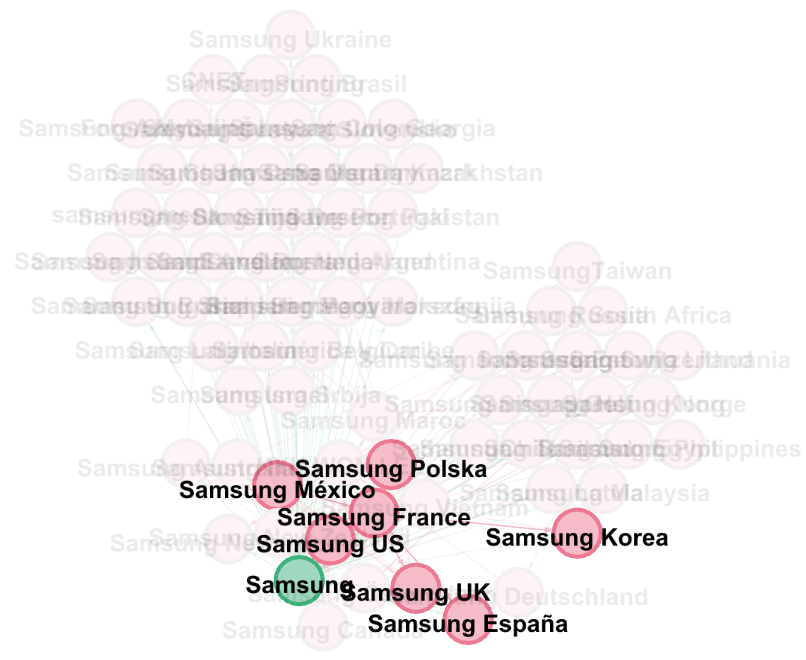
\includegraphics[width=0.6\textwidth]{photos-files/section8/mikro.png}
	\end{center}
	\par
	Κανάλι με μεσαίου σκορ Clustering Coefficient:
	\begin{center}
		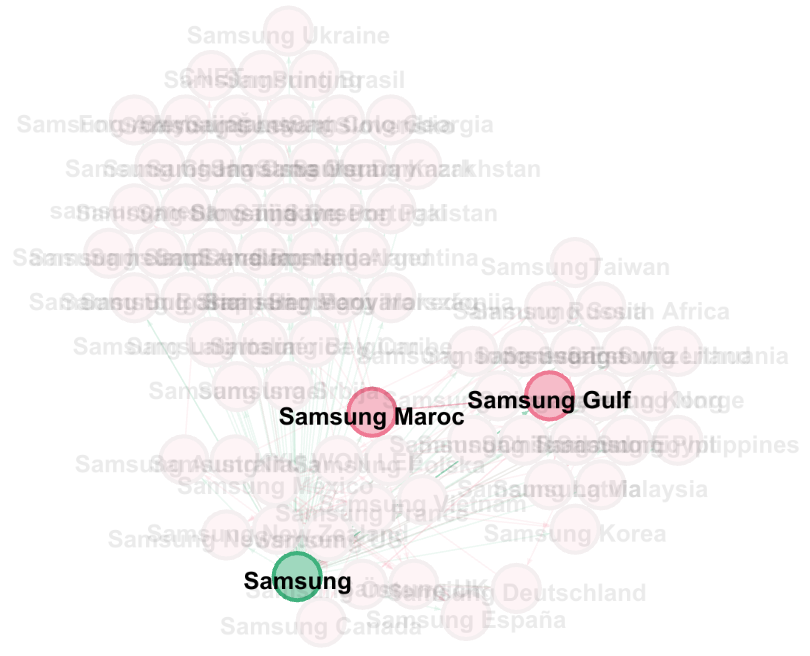
\includegraphics[width=0.6\textwidth]{photos-files/section8/meseo.png}
	\end{center}
	\newpage
	Κανάλι με υψηλό Clustering Coefficient:
	\begin{center}
		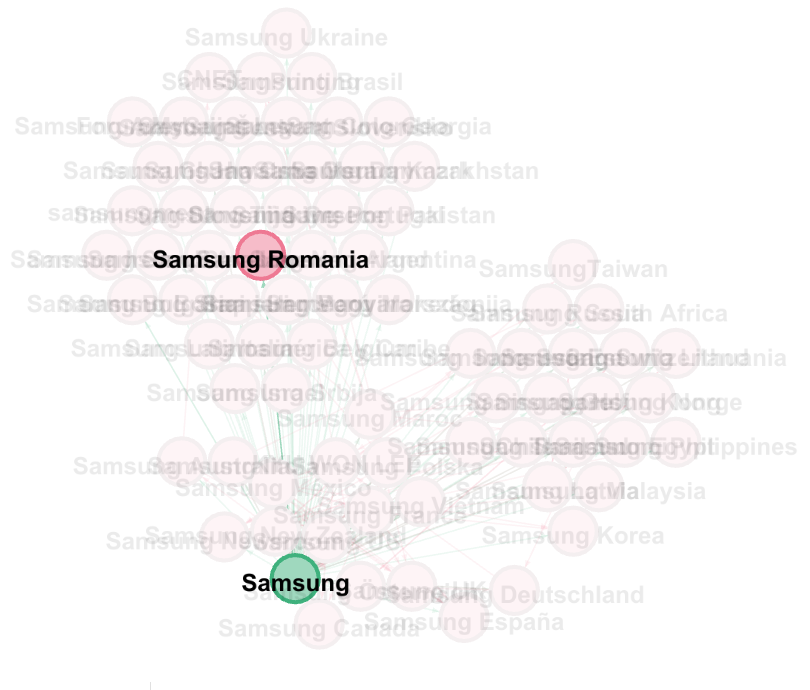
\includegraphics[width=0.6\textwidth]{photos-files/section8/megalo.png}
	\end{center}
	Τα σχήματα αυτα δημιουργήθηκαν ανα ομάδες με κρητίριο το Clustering Coefficient και γι'αυτό φαίνονται 3 ομαδοποιήσεις. Σε κάθε διαφορετική εικόνα, έχουμε με πιο έντονο χρώμα τους κόμβους που συνδέονται μεταξύ τους ανάλογα με το ύψος του Clustering Coefficient.
	
	\newpage
	\subsection{Existence of the Triadic Closure Phenomenon in the Friendship Neighborhood}
	Η ύπραξη τριαδικής κλειστότητας σε Friendship Neighborhood είναι ένα φαινόμενο το οποίο παρακολουθειται σε βάθος χρόνου. Για παράδειγμα στη πραγματική ζωη, όταν δύο άτομα(που δεν γνωρίζονται αρχικα) κάνουν παρέα με ένα κοινο άτομο, είναι πολύ πιθανό πως μελλοντικά, το κοινό αυτο άτομο που γνωρίζουν θα τους φέρει σε επαφή ώστε να γνωριστούν. Έτσι διευρίνεται ο κύκλος ενός ατόμου μέσω "Friendship Neighborhoods" απο τον κύκλο ενός φίλου. Όσον αφορά το δίκτυο το οποίο εξετάζουμε, αυτό μπορεί να γίνει τοσο εύκολα όπως το σενάριο που περιγράψαμε προηγουμένως. Για παράδειγμα βλέπουμε πιο κάτω τα κανάλα Samsung Lithuania και Samsung Latvia τα οποία συνδέονται με το κοινό κανάλι Samsung.
	\begin{center}
		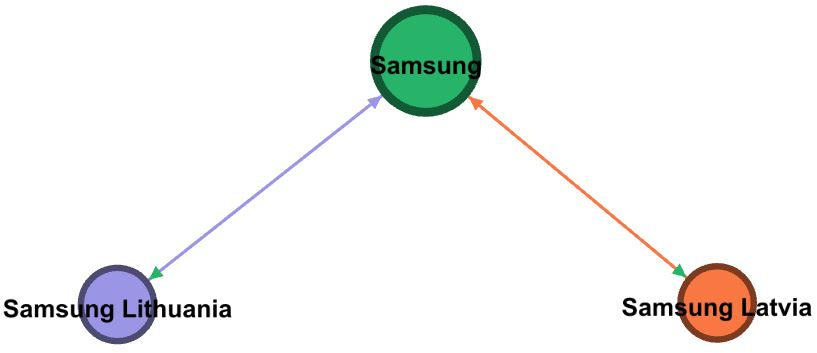
\includegraphics[width=0.7\textwidth]{photos-files/section8/8.4_with_2_edges.JPG}
	\end{center}
	Αυτό σημαίνει πως το κανάλι Samsung έχει ως featured channels τα Samsung Lithuania και Samsung Latvia και ταυτόχρονα αυτα τα δύο έχουν ως featured channel το κανάλι Samsung. Επομένως αφού οι χρήστες του καναλιού Samsung Lithuania βλέπουν προτεινόμενα βίντεο για το κανάλι Samsung, και οι χρήστες του καναλιού Samsung βλέπουν προτεινόμενα βίντεο για το κανάλι Samsung Latvia, τότε θα είναι πιθανό οι χρήστες του Samsung Lithuania να ενδιαφέρονται για τα βίντεο του Samsung Latvia.
	\par
	Αυτό ισχύει και για την αντίθετη περίπτωση ξεκινόντας απο το κανάλι Samsung Latvia και καταλήγοντας στο κανάλι Samsung Lithuania.
	
	\newpage
	Άρα μπορεί να γίνει η σύνδεση με τα featured channels που περιγράψαμε όπως φαίνεται στην πιο κάτω εικόνα.
	\begin{center}
		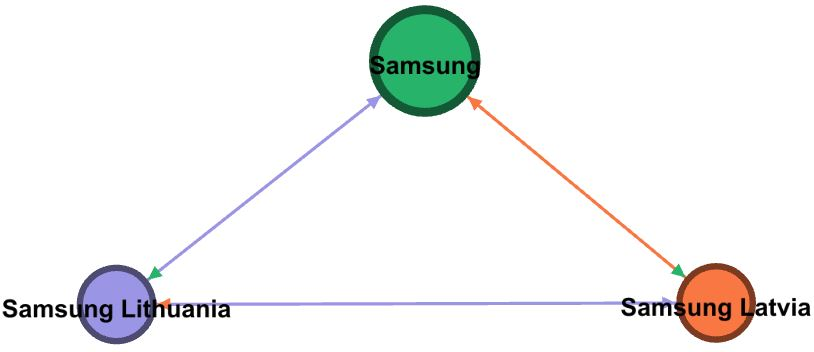
\includegraphics[width=0.7\textwidth]{photos-files/section8/8.4_with_3_edges.JPG}
	\end{center}
	Το αποτέλεσμα μπορεί να είναι όπως φαίνεται στην τελευταία εικόνα χωρίς να είναι βέβαια απαραίτητη η αμφίδρομη σύνδεση.
	\label{chap:clustering_effects_8}
	
	
	\newpage
	\section{Bridges and Local Bridges}
	Γέφυρα ή αλλίως Bridge στην αγγλική ορολογία θεώρούμε την μοναδίκη ακμή η οποία συνδέει 2 κόμβους όπου κάθε ενας απο αυτόυς ανήκει σε ένα μία διαφορετική γείτονία(ειδικότερα οταν η κάθε γειτονιά έχει πιο ισχυρούς δεσμους μεταξύ της). Με άλλα λόγια, αν η ακμή αυτη διαγραφτεί, θα χωρίσει το δίκτυο στο οποίο ανήκει στα δύο.
	\begin{center}
		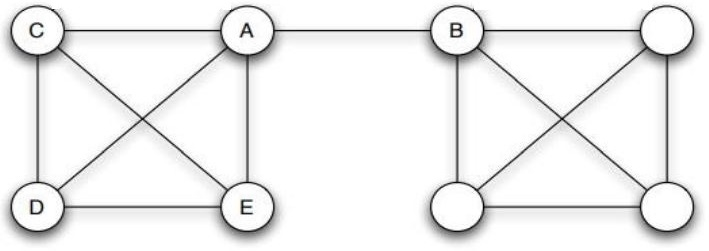
\includegraphics[width=0.6\textwidth]{photos-files/section9/bridge_example.jpg}
	\end{center}
	\vspace{12pt}
	Έστω πως έχουμε παρόμοιο δίκτυο με το προηγούμενο, μόνο που η σύνδεση των δύο κόμβων που αποτελέι την ένωση των δύο κοινοτήτων δεν είναι η μοναδική όπως πιο κάτω:
	\begin{center}
		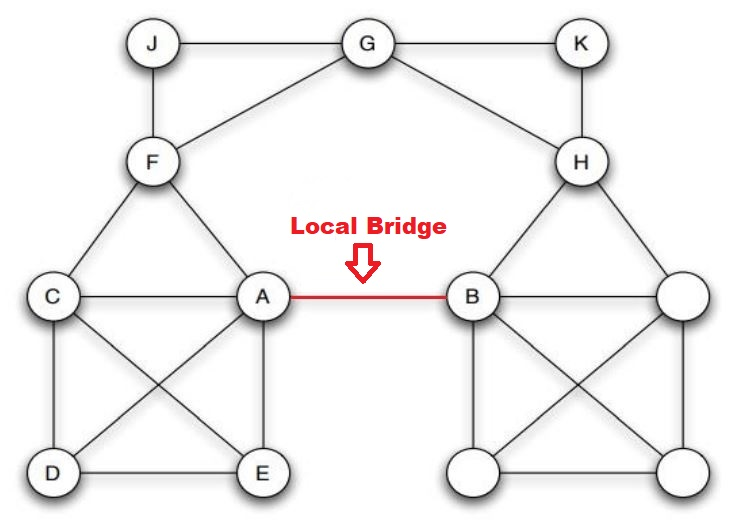
\includegraphics[width=0.6\textwidth]{photos-files/section9/local_bridge_example.jpg}
	\end{center}
	\vspace{12pt}
	Στη περίπτωση δηλαδηή όπου υπάρχουν περισσότερρες απο μία ακμές θεωρούμε ως Local Bridge την ακμή όπου η διαγραφή της θα αυξήσει την απόσταση μεταξύ των 2 κόμβων που συνέδεε.
	
	\newpage
	Στο δικτυο που εξετάζουμε... \textcolor{red}{afinnw piso ta ipoloipa j paw parakatw}
	\label{chap:bridges_and_local_bridges_9}
	
	
	
	\newpage
	\section{Gender and homophily}
	\label{chap:gender_and_homophily_10}
	
	
	
	
	\newpage
	\section{Graph Density}
	Το Graph density είναι μια μετρική για την συνδεσιμότητα των κόμβων σε ένα γράφημα. Υπολογίζεται με το γινόμενο των ακμών που έχει το δίκτυο προς τον συνολικό αριθμό ακμών που θα μπορούσε να έχει εαν όλοι οι κόμβοι ήταν συνδεδεμένοι με όλους. Στο δίκτυο μας όπως είδαμε και στην ενοτητα 4 για τα Βαικά στοιχεία Δικτύου, ο αριθμός κόμβων είναι 76 και ο αριθμός ακμών είναι 149. Άρα αφού πρόκειται για κατευθυνόμενο γράφο, ο συνολικός αριθμος ακμών που θα μπορούσε να έχει το δίκτυο μας είναι 76*75 = 5700. Επομένως το Graph Density για το δίκτυο μας είναι 149 / 5700 = 0.026. Πράγματι αυτό επιβεβαιώνεται μέσω του Gephi.
	\begin{center}
		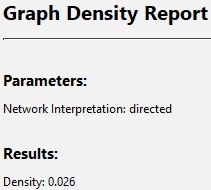
\includegraphics[width=0.3\textwidth]{photos-files/section11/density.JPG}
	\end{center}Το αποτέλεσμα που βρήκαμε είναι αρκετά μικρος αριθμός. Λογικό, αφού αν ανατρέξουμε στο δίκτυο μας θα δούμε πως υπάρχει ενα αρκετά μεγαλο ποσοστό κόμβων που είναι ενωμένοι μόνο με έναν άλλο. Αυτό φαίνεται μέσω του Total Degree που έχουν οι κόμβοι αυτοί, που είναι ίσο με 1.
	\begin{center}
		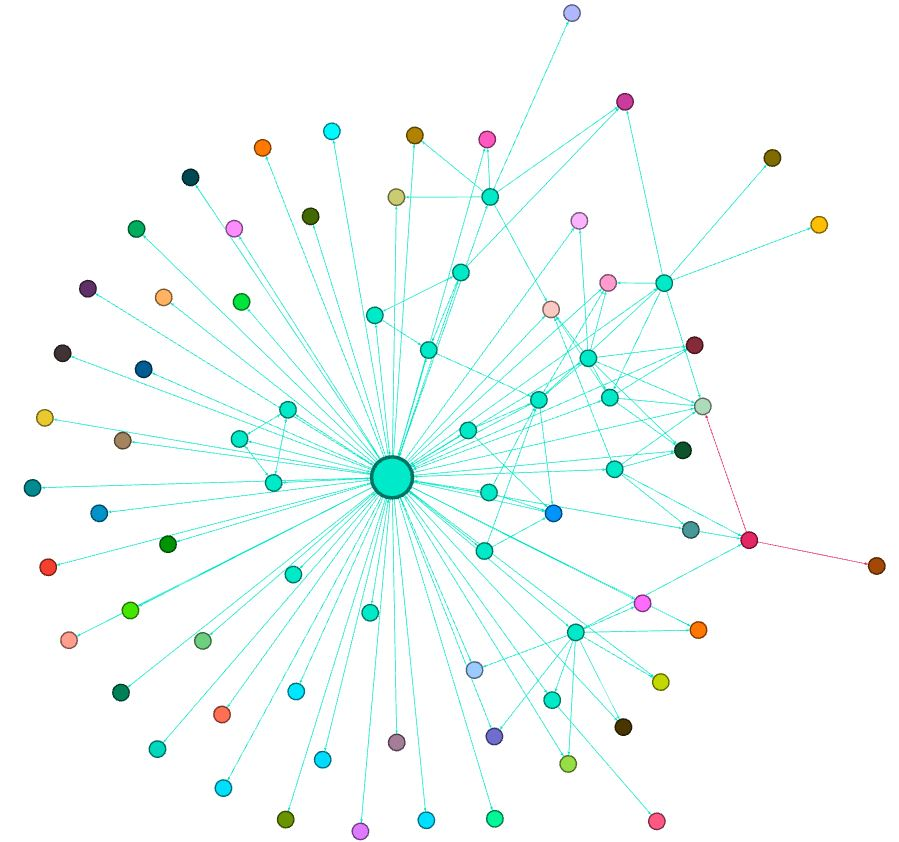
\includegraphics[width=0.55\textwidth]{photos-files/section11/our_sparse_graph.JPG}
	\end{center}
	
	\textcolor{red}{an prolavw enna pw pramata opos lalei j o koumparos sto diko tou sto sl. 49 j 50 gia to Graph Density}
	%Στο σημείο αυτό μπορούμε να συγκρίνουμε την πυκνότητα του δικτύου μας 
	\label{chap:graph_density_11}
	
	
	
	
	\newpage
	\section{Community Structure(Modularity)}
	Στο σημείο αυτό, μπορούμε να δούμε πως το δίκτυο μας διαχωρίζεται σε communities ουτως ώστε να εξάγουμε κάποια συμπεράσματα. Αυτό μπορεί να γίνει με τη χρήση του Modularity μέσω των Statistics του Gephi ωστα να δούμε τα διαφορετικά Communities που σχηματίζονται. Τρέχοντας λοιπόν το στατιστικό Modularity, εμφανίζεται το πιο κάτω παράθυρο.
	\begin{center}
		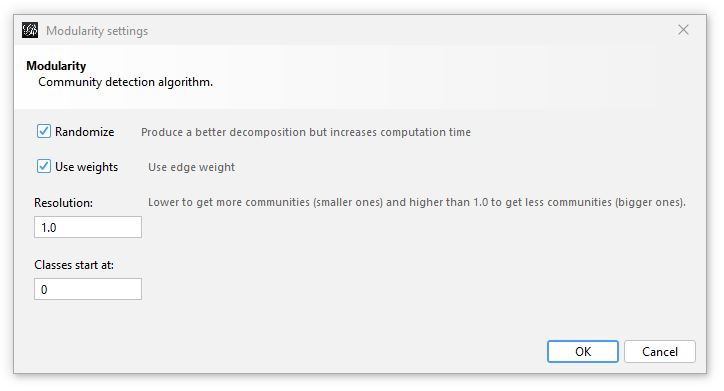
\includegraphics[width=0.8\textwidth]{photos-files/section12/eisagogi_modularity_twn_statistics.JPG}
	\end{center}
	Όπως βλέπουμε, υπάρχουν ορισμένες επιλογές οι οποίες μπορούν να ληφθουν υπόψην όπως το randomize, το βάρος των ακμών, το Resolution και η αρχική τιμή απο την οποία θα ξεκινάει η αρίθμηση των κόμβων για τη μετρικη που θα παραχθεί. Στα πλαίσια της ανάλυσης μας ενδιαφέρει το Resolution αφου αυτό είναι που διαμορφώνει το πλήθος των communities ανάλογα με την τιμή που θα πάρει(μικροτερες τιμες έχουν αποτέλεσμα πιο πολλα communities και μεγαλύτερες τιμες λιγότερα communities). Να σημειωθεί επίσης πως το βάρος των ακμών είναι ίδιο σε όλο μας το δίκτυο ενω ο βαθμος στον οποίο επηρεαζει τα αποτελέσματα μας είναι ελάχιστος εως μηδαμινος σύμφωνα με μετρήσεις που έχουν πραγματοποιηθεί. Επομένως αφού το Resolution καθορίζει τα αποτελέσματα μας, μετα απο αρκετές δοκιμασίες που κάναμε για να καταλάβουμε πως διαμορφώνονται τα communities καταλήξαμε στα πιο κάτω αποτελέσματα.
	
	\textcolor{red}{ara mporoume na dume pws eksaplonontai oi tasis j ta new dedomena klp apo xora se xora j meta se olokliro to kosmo}
	
	\newpage
	\subsection{Community Structure - Modularity Resolution 0.1}
	Με Resolution 0.1 έχουμε Modularity 0.283 ενώ δημιουργoύνται 20 communities διαφόρων μεγεθών καθώς τα μικρότερα αποτελούνται απο 1 μονο κόμβο(7 communities) ενω το μεγαλύτερο απο 26. Όπως βλέπουμε υπάρχει μεγάλη διαφορά στο πλήθος των communities καθώς επίσης και μεγάλη κατανομή.
	\vspace{12pt}
	\begin{center}
		\begin{adjustbox}{valign=t}
			\includegraphics[width=0.25\textwidth]{photos-files/section12/0.1/report.JPG}
		\end{adjustbox}
		\hfill
		\begin{adjustbox}{valign=t}
			\includegraphics[width=0.5\textwidth]{photos-files/section12/0.1/no_label_layout.png}
		\end{adjustbox}
	\end{center}
	
	Να πούμε επίσης πως σε μικρές ομαδοποιήσεις τα κανάλια απο τα οποία αποτελόυνται είναι απο χώρες που βρίσκονται γεωγραφικά κοντά ή στην ίδια ήπειρο όπως για παράδειγμα:
	
	\vspace{12pt}
	\vspace{12pt}
	\vspace{12pt}
	\begin{minipage}{0.6\textwidth}
		Το community με ροζ χρώμα αποτελείται απο τα κανάλια Samsung Latvia, Samsung Lithuania, Samsung Estonia.
			%\begin{center}
				%\includegraphics[width=0.8\textwidth]{photos-files/section4/ate.JPG}
			%\end{center}
	\end{minipage}
	\hspace{0.05\textwidth}
	\begin{minipage}{0.3\textwidth}
		\includegraphics[width=1.0\textwidth]{photos-files/section12/0.1/lith_est_latv_community.png}
	\end{minipage}
	
	\vspace{12pt}
	\vspace{12pt}
	\vspace{12pt}
	\begin{minipage}{0.6\textwidth}
		Το community με μπλε χρώμα αποτελείται απο τα κανάλια Samsung Switzerland, Samsung Deutschland(Γερμανία), Samsung Osterreich(Αυστρία).
		%\begin{center}
		%\includegraphics[width=0.8\textwidth]{photos-files/section4/ate.JPG}
		%\end{center}
	\end{minipage}
	\hspace{0.05\textwidth}
	\begin{minipage}{0.3\textwidth}
		\includegraphics[width=1.0\textwidth]{photos-files/section12/0.1/swi_ost_deu_community.png}
	\end{minipage}
	
	\vspace{12pt}
	\vspace{12pt}
	\vspace{12pt}
	\begin{minipage}{0.6\textwidth}
		Το community με πράσινο χρώμα αποτελείται απο τα κανάλια Samsung New Zealand, Samsung Singapore, Samsung Malaysia, Samsung Hong Kong, Samsung Taiwan, Samsung Philippines, Samsung Thailand και Samsung Indonesia. Τα κανάλια αυτά είναι απο χώρες οι οποίες μπορει να μην είναι τόσο κοντά όπως στις προηγούμενες περιπτώσες που είδαμε αλλά ανήκουν σχεδόν όλες στην ίδια ήπειρο εκτός απο την Νεα Ζηλανδία.
		%\begin{center}
		%\includegraphics[width=0.8\textwidth]{photos-files/section4/ate.JPG}
		%\end{center}
	\end{minipage}
	\hspace{0.05\textwidth}
	\begin{minipage}{0.3\textwidth}
		\includegraphics[width=1.0\textwidth]{photos-files/section12/0.1/asia_community.png}
	\end{minipage}

	\vspace{12pt}
	\vspace{12pt}
	\vspace{12pt}
	\begin{minipage}{0.6\textwidth}
		Το community με γαλάζιο χρώμα αποτελείται απο τα κανάλια Samsung South Africa, Samsung Egypt, Samsung Maroc, samsungmena, Samsung Gulf. Σε αυτό το community βλέπουμε κανάλια απο χώρες της Βορείου Αφρικής(Ηπείρου) και της Μέσης Ανατολής.
		%\begin{center}
		%\includegraphics[width=0.8\textwidth]{photos-files/section4/ate.JPG}
		%\end{center}
	\end{minipage}
	\hspace{0.05\textwidth}
	\begin{minipage}{0.3\textwidth}
		\includegraphics[width=1.0\textwidth]{photos-files/section12/0.1/vorioAfriki_middleEast.png}
	\end{minipage}
	
	\vspace{12pt}
	\vspace{12pt}
	\vspace{12pt}
	\begin{minipage}{0.6\textwidth}
		Το community με έντονο ροζ χρώμα αποτελείται απο τα κανάλια Samsung South Canada, Samsung Chile, Samsung Mexico. Σε αυτό το community βλέπουμε κανάλια απο χώρες της Αμερικής(Ηπείρου).
		%\begin{center}
		%\includegraphics[width=0.8\textwidth]{photos-files/section4/ate.JPG}
		%\end{center}
	\end{minipage}
	\hspace{0.05\textwidth}
	\begin{minipage}{0.3\textwidth}
		\includegraphics[width=1.0\textwidth]{photos-files/section12/0.1/ameriki_ipiros.png}
	\end{minipage}
	
	\vspace{12pt}
	\vspace{12pt}
	\vspace{12pt}
	Τα υπόλοιπα communities αποτελούνται απο κανάλια στα οποία οι χωρες που προέρχονται δεν εχουν κάποια σχεση ή ειναι communities με ένα και μοναδικό κανάλι.

	%\vspace{12pt}
	%\vspace{12pt}
	%\vspace{12pt}
	%\begin{minipage}{0.6\textwidth}
		%This is some text that you want to have next to the picture. You can write as much text as you need %within this minipage.
	%\end{minipage}
	%\hspace{0.05\textwidth}
	%\begin{minipage}{0.3\textwidth}
		%\includegraphics[width=0.5\textwidth]{example-image-a}
	%\end{minipage}
	
		
	\newpage
	\subsection{Community Structure - Modularity Resolution 0.5}
	Με Resolution 0.5 εχουμε Modularity 0.396 ενώ δημιουργoύνται 8 communities μεγέθους 3, 3, 5, 5, 5, 10, 10 και 35 κόμβων. Ακολουθουν τα ποσοστά σε σχέση με το μέγεθος του δικτύου καθώς επίσης οι μετρήσεις και ο τρόπος διάταξης του συγκεκριμένου community structure.
	
	\vspace{12pt}
	\vspace{12pt}
	\begin{center}
		\begin{adjustbox}{valign=t}
			\includegraphics[width=0.25\textwidth]{photos-files/section12/0.5/report.JPG}
		\end{adjustbox}
		\hfill
		\begin{adjustbox}{valign=t}
			\includegraphics[width=0.3\textwidth]{photos-files/section12/0.5/pososta.JPG}
		\end{adjustbox}
	\end{center}
	
	\vspace{12pt}
	\vspace{12pt}
	\begin{center}
		\includegraphics[width=0.6\textwidth]{photos-files/section12/0.5/no_label_layout.JPG}
	\end{center}
	
	\newpage
	Στο σημείο αυτο και με τα στατιστοικα που έχουμε πάρει, καταλαβαίνουμε προφανως πως ο αριθμος των communities έχει μειωθεί, δεν υπάρχουν πλεον ατομικά communities αφου έχουν συγωνευθει με άλλα, ενω ταυτόχρονα ορισμένα άλλα κανάλια έχουν εντααχθεί σε πρηγούμενα communities που είχαμε στη προηγούμενη υποενότητα με Resolution 0.1. Πιο συγκεκριμένα έχουμε:
	
	\vspace{12pt}
	\vspace{12pt}
	\vspace{12pt}
	\begin{minipage}{0.6\textwidth}
		Στο community όπου προηγουμένως αποτελείτω απο τα κανάλια Samsung New Zealand, Samsung Singapore, Samsung Malaysia, Samsung Hong Kong, Samsung Taiwan, Samsung Philippines, Samsung Thailand και Samsung Indonesia πλέον έχουν προστεθεί τα κανάλια Samsung Vietnam και ForumMySamsung. Το γεγονός αυτο δεν μας εκπλήσσει αφού πάλι πρόκειται για κανάλια που απευθύνονται σε κοινό απο ασιατικές χώρες, προφανως για το Βιετναμ αλλα και για το καναλι ForumMySamsung αφου όπως είδαμε το περιεχόμενο του είναι στα Βιετναμέζικα. Δίπλα φάίνεται η καινούργια μορφή του συγκεκριμένου community.
		%\begin{center}
		%\includegraphics[width=0.8\textwidth]{photos-files/section4/ate.JPG}
		%\end{center}
	\end{minipage}
	\hspace{0.05\textwidth}
	\begin{minipage}{0.3\textwidth}
		\includegraphics[width=1.15\textwidth]{photos-files/section12/0.5/vietnam_j_forum.png}
	\end{minipage}
	
	
	
	
	
	
	
	
	
	
	
	
	
	
	
	
	
	
	
	
	
	
	
	
	
	
	
	
	
	
	\newpage
	\subsection{Community Structure - Modularity Resolution 0.9}
	Με Resolution 0.9 εχουμε Modularity 0.399 και δημιουργoύνται 7 communities μεγέθους 3, 3, 5, 10, 10, 11 και 34 κόμβων. Ακολουθουν τα ποσοστά σε σχέση με το μέγεθος του δικτύου καθώς επίσης οι μετρήσεις και ο τρόπος διάταξης του συγκεκριμένου community structure.
	
	\vspace{12pt}
	\vspace{12pt}
	\begin{center}
		\begin{adjustbox}{valign=t}
			\includegraphics[width=0.25\textwidth]{photos-files/section12/0.96/report.JPG}
		\end{adjustbox}
		\hfill
		\begin{adjustbox}{valign=t}
			\includegraphics[width=0.3\textwidth]{photos-files/section12/0.96/pososta.JPG}
		\end{adjustbox}
	\end{center}
	
	\vspace{12pt}
	\begin{center}
		\includegraphics[width=0.6\textwidth]{photos-files/section12/0.96/no_label_layout.JPG}
	\end{center}
	
	Στη παρούσα φάση όπως και πριν, βλέπουμε να συγωνέυονται ακόμη περισσότερο οι κόμβοι σε πιο μεγάλα communities. Πλέον φαίνεται να ξεπερναμε το μοντέλο της ομαδοποιησης κατα χώρες. Αυτό δεν μπορούμε να πουμε πως είναι κακό αφού το κρητήριο με το οποίο υπάρχουν οι ακμές στο δίκτυο μας δεν καθορίζεται απο τις χώρες στις οποίες βρίσκονται τα κανάλια αλλα παίζει σίγουρα σημαντικό ρόλο αφού όπως είδαμε γίνονται ομαδοποιήσεις ανάλογα με την περιοχή στην οποία βρίσκονται γεωγραφικά τα κανάλια και τη γλώσσα στην οποία μιλούν. Επομένως, μετα απο οσα προηγήθηκαν, καταλαβάινουμε οτι κάθε Resolution επαιξε το δικό του ρόλο ώστε να εξάγουμε τα συμπεράσματα αυτά.
	\label{chap:community_structure_(modularity)_12}
	
	
	
	
	
	
	
	
	
	
	
	
	
	
	
	
	
	
	
	
	
	
	
	
	
	\newpage
	\section{PageRank}
	\label{chap:PageRank_13}
	Το PageRank αποτελέι έναν αλγόριθμο ο οποίος αρχικά αναπτύχθηκε απο την Google για την κατάταξη των ιστοσελίδων με σκοπό την καλύτερη και πιο αποτελεσμάτική εμφάνηση τους στις αναζητήσεις των χρηστών. Ο αλγόριθμοςς αυτός εφαρμόζεται και στην ανάληση δικτύων  αφου χρησιμοποιείται για την μέτρηση της σημασίας ή της επιρροής των κόμβων σε ενα δίκτυο με την ανάθεση αριθμητικής τιμής η οποία αντιπρωσοπεύει την σημαντικότητα ενός κόμβου στο δίκτυο. Ο υπολογισμός του PageRank σε ενα δίκτυο γίνεται με βάση τον αριθμό και την ποιότητα των συνδέσμων σε ένα κόμβο ενώ επίσης κόμβοι με υψηλότερη τιμή θεωρούνται σημαντικότεροι. Πιό κάτω, βλέπουμε τις μετρήσεις των κόμβων για το δύκτυο μας μεσω του Gephi.
	
	\begin{center}
		\begin{adjustbox}{valign=t}
			\includegraphics[width=0.35\textwidth]{photos-files/section13/pagerank_1.JPG}
		\end{adjustbox}
		\hfill
		\begin{adjustbox}{valign=t}
			\includegraphics[width=0.35\textwidth]{photos-files/section13/pagerank_2.JPG}
		\end{adjustbox}
	\end{center}
	
	\newpage
	Όπως ήταν αναμενόμενο για άλλη μια φορά στην κορυφή βρίσκεται το κανάλι Samsung. Τα υπόλοιπα κανάλια, τα βλέπουμε να ακολουθούν με αρκετά μεγάλη διαφορά σε σχέση με το σκορ που σημειώνει το πρώτο κανάλι. Επομένως σύμφωνα με το PageRank το πιο σημαντικό κανάλι είναι της Samsung. Εκτός απο αυτό, παρατηρούμε πως οι τιμές των υπόλοιπων κόμβων είναι αρκετά κοντινές ενω επίσης συναντόνται ομαδοποιήσεις. Για να δουμε σχηματικά τη δαφορά, μπορούμε να διαχωρίσουμε και να ταξινομήσπυμε τους κόμβους ως προς τη μετρική που εξετάζουμε. Τα αποτελέσματα ακολουθούν πιο κάτω.
	\vspace{12pt}
	\begin{center}
		\includegraphics[width=0.7\textwidth]{photos-files/section13/layout.JPG}
	\end{center}
	\vspace{12pt}
	Ο σχηματισμός έγινε με βάση το Dual Circle Layout ενώ ο χρωματισμός και η σειρά των κόμβων στον εξωτερικό κύκλο με βάση το PageRank. Με δεδομένο οτι υπάρχει ενας μονο κόμβος με σημαντικα μεγαλο σκορ βάλαμε λοιπόν ενα μόνο κόμβο στο εσσωτερικό του σχήματος οπότε δεν μπορεί να σχηματιστέι κάποιος εσωτερικός κύκλος. Με αυτό το τρόπο όμως μπορούμε εύκολα να διακρίνουμε τους κόμβους που έχουν τις λιγότερες συνδέσεις και επομένως το μικρότερο PageRank αφού ενόνονται μόνο με έναν κόμβο. Μιλάμε βέβαια για τους κόμβους με τον πορτοκαλί χρωματισμό. Έτσι συνεχίζοντας στον κύκλο μπορούμε να δούμε πως αυξάνεται το PageRank με βάσει τον αριθμό των συνδέσεων των κόμβων.
	
	Τα πιο πάνω αποτελέσματα οφείλονται στο οτι οι κόμβοι μεταξύ τους δεν έχουν την ιδιάιτερη σχέση όπως έχει ο κόμβός που αντιπροσωπεύει το κανάλι της Samsung με όλους τους υπόλοιπους αφου όπως είπαμε και στην αρχη, η σχέση με την οποία συνδέονται τα κανάλια είναι μέσω των featured channels ξεκινόντας απο έναν μόνο seeder.
	
	
	
	\newpage
	\section{Συμπεράσματα}
	
	\textcolor{red}{paizei rolo h glossa ara j xora j oi diplanes xores pou mporei na miloun thn idia glossa}
	
	\label{chap:simperasmata_14}	
\end{document}
